\def\year{2016}\relax
%File: formatting-instruction.tex
\documentclass[letterpaper]{article}
\usepackage{aaai16}
\usepackage{times}
\usepackage{helvet}
\usepackage{subfig}
\usepackage{amssymb}
\usepackage{enumitem}
\usepackage{amsmath}
\usepackage{pifont}
\usepackage{multirow}
\usepackage{hyperref}
\usepackage[table,xcdraw]{xcolor}
\usepackage[normalem]{ulem}
\useunder{\uline}{\ul}{}
\usepackage{courier}
\usepackage{graphicx}
\usepackage{epsfig}
\usepackage{xr}
\newcommand{\xmark}{\ding{55}}%
\newcommand{\starmark}{\ding{72}}%
\frenchspacing
\setlength{\pdfpagewidth}{8.5in}
\setlength{\pdfpageheight}{11in}
\pdfinfo{
/Title (Learning Topical Social Sensor on Twitter)
/Author (Author1, Author2, Author3}
\setcounter{secnumdepth}{1}  

\newcommand{\eat}[1]{}
\newcommand{\rev}[1]{{\color{blue}{#1}}}

 \begin{document}
% The file aaai.sty is the style file for AAAI Press 
% proceedings, working notes, and technical reports.
%
\title{Learning Topical Social Sensors}
\author{Authors\\
Affiliations
}
\maketitle
\begin{abstract}
%!TEX root = icwsm2016.tex

Social media sources such as Twitter represent a massively distributed
social sensor of a \eat{rich underlying topic space}\rev{kaleidoscope of topics} ranging from social and
political events to entertainment and sports news.  \eat{However, given the
continual evolution of social media content, querying for content from
individual users or containing certain keywords or hashtags is often
insufficient to retrieve the vast range of topical content available.}
\rev{We note, however, that due to the overwhelming volume of content, 
it can be difficult to spot novel and significant topics within a broad theme 
in a timely fashion -- 
such as \#obamacare or a recent \#twochild policy in China. }
\rev{This paper propose a scalable and practical method to automatically construct social sensors for generic topics.}\eat{To automate generic social sensor construction,} we
%address the task of automatically learning topical
%social sensors that generalize to future unseen content
%As a simple
%but critical insight, we leverage hashtags as proxies for topical
%content to automatically label a vast corpus of social media with only
%a small number of topical hashtags that users can easily curate.  With
%this labeled data in hand, we train a supervised learner to identify
train a supervised learner to identify topical content 
\rev{from millions of features capturing content, user and social interactions on Twitter.}
\eat{over a large
feature space given a small set of seed hashtags as proxies for
topic labels.}  
On a corpus of approximately 1 billion English Tweets
% or 40TB of Twitter data?  does not seem like 1 billions tweets though!
collected from the Twitter
streaming API during 2013 and 2014 and learning for 10 diverse \rev{themes}\eat{topics}
ranging from social issues to celebrity deaths to the ``Iran nuclear
deal'', we empirically show that our learned social sensor
automatically generalizes to unseen future content 
\eat{(including content with no hashtags)}
with high ranking and precision scores.  Furthermore, 
we provide an extensive analysis of features and feature types across
different topics that reveals, for example, that (1)~largely
independent of topic, simple terms are the most informative feature
followed by location features and that (2)~the number of unique
hashtags and tweets by a user correlates more with their
informativeness than their follower or friend count.  In summary, this
work provides a novel, effective, and efficient way to learn topical
social sensors from a seed set of hashtags requiring minimal user
curation effort and offering strong generalization to future topical content.


%Twitter represents a massively distributed social sensor of a rich
%underlying topic space that drives its content generation.  Yet
%Twitter content is so diverse, decentralized, and dynamic in nature,
%that it is hard to automatically aggregate this topical content.  To
%address this need, we provide a novel way of learning topical social
%sensors on Twitter that learn from a provided set of topical hashtags
%and generalize to identify topical tweets with previously unseen tags.
%These learning social sensors leverage a variety of user-based,
%hashtag-based, term-based, and location-based features for
%distinguishing topical from non-topical tweets; we further analyze
%these features to understand which features are most useful and why.
%We further assess general global topical trends and how our learning
%sensors are able to follow these trends by drawing from a rich variety
%of sources on the Twittersphere to enable a first generation of
%learning social sensors for Twitter.

\end{abstract}

\section{Introduction}
%!TEX root = document.tex

%start with a clean argument then fill in details.  
%Motivation is mostly the same, 
%contributions are different... we combine recent ideas on learning social sensors 
%	(you need to cite / cover what these ideas are to indicate what you're combining / building on -- perhaps being clear to point out that no single paper did everything you are doing) and then claim that beyond a general performance analysis of the framework over a variety of topics and a long-term dataset (not done previously?) 
%a key objective of the work is to provide a comprehensive longitudinal feature analysis to investigate XXX



\label{sec:introduction}
% Motivation
Social media sites such as Twitter present a double-edged sword for
users.  On one hand these sources contain a vast amount of novel and
topical content that challenge traditional news media sources in terms
of their timeliness and diversity.  Yet on the other hand they also
contain a vast amount of spam and otherwise low-value content for most
users' information needs where filtering out irrelevant content is
extremely time-consuming.  Hence, while it is widely acknowledged that
social media sources can be used as topical content sensors (indeed,
an entire European Union project was focused on related ``Social Sensor''
research\footnote{\texttt{http://www.socialsensor.eu/}}.),
automatically learning high-precision sensors (i.e., ranking and
retrieval methods) for arbitrary topics that generalize to future
unseen content have been addressed recently only by a handful of researchers \citep{lin2011smoothing,yang2014large,magdy}.
% and comprises the key problem we seek to address in this paper.

% Contribution 
% 1. One sentense: what do we do, combine, provide supervised learning, none of them has done all
% 2. What did existing works do?
% 3. How did we approach the problem? Build on existing ideas or expanded them?
% 4: What is the differences?

In this work, we coalesce recent ideas on learning social sensors for general topic detection. We expand these works to learn a generalizable supervised method with minimal user curation for detecting and ranking topical content over a variety of topics and on a long-term dataset. We believe that none of the earlier works covers all the aspect of the work that is presented here. 
%We contribute a supervised method for training
%social sensors with minimal user curation by using a small seed set of
%hashtags as topical proxies for automatic supervised data labeling. This works is built on the existing literature on detection and tracking general topics from social media \citep{lin2011smoothing,yang2014large,magdy}.
Recently, \citep{lin2011smoothing,yang2014large,magdy} have explored use of social media sensors for detection and/or tracking of general topics from Twitter. One of the key challenges on dealing with general topics and large number of tweets is automatic labeled data aquisition. \cite{lin2011smoothing} discusses automatic labeling of tweets by using one hashtag as topic proxy. \cite{magdy} uses a user-defined query to label tweets and \cite{yang2014large} takes a co-training approach based on embedded URLs in the tweet and tweet text to label tweets. We build and extend on \citep{lin2011smoothing}'s idea of automatic labeling of tweets, however we choose a set of hashtags for each topic instead of a single hashtag which we will show to be imperative for evaluating generalization. To learn social sensors for general topic detection, \citep{lin2011smoothing} uses information retrieval method (language models), \cite{yang2014large} take advantage of topic modeling techniques and \cite{magdy} applies SVM classifier. Here, we leverage various supervised learning methods for the purpose of detection and ranking of topical content. However, we present a unique method for splitting hashtags and Twitter data that encourages generalization to new unseen future content. 
%The methodologies mentioned in the literature use various sets of feature including hashtags, unigrams, bigrams, mentions, users, byte 4grams. We extract the main features of hashtags, mentions, users, unigrams. In addition, we add location as another set of features which we show later in feature analysis that location is the second most important feature for detection of topical content and some of the topics are quite localized geographically. To address general topic detection from social media, \cite{lin2011smoothing} uses information retrieval method (language models), \cite{yang2014large} take advantage of topic modeling techniques and \cite{magdy} uses SVM classifier. Here, we leverage various supervised learning methods for the purpose of detection and ranking of topical content. However, we present a unique method for splitting hashtags and Twitter data that encourages generalization to new unseen future content. 
Then we proceed to train supervised classification and ranking methods
to learn topical content from a large feature space of source users
and their locations, terms, hashtags, and mentions.  On a corpus of
over 800 million English Tweets collected from the Twitter streaming
API during 2013 and 2014 and covering 10 diverse topics ranging from
"social issues" to "celebrity deaths" to the "Iran nuclear deal'', we
empirically show that two simple and efficiently trainable methods ---
logistic regression and naive Bayes --- generalize well to unseen
future topical content (including content with no hashtags) in terms
of their mean average precision (MAP) and Precision@$n$ for a range of
$n$. Our results suggest that these
sensors generalize well to unseen future topical content and provide a
novel paradigm for the extraction of high-value content from social
media.  Furthermore, we show that terms and locations are among the most
useful features --- surprisingly more so than hashtags, even though
hashtags were used to label the data.  And perhaps even more
surprisingly, the number of unique hashtags and tweets by a user
correlates more with their informativeness than their follower or
friend count.
 
In summary, we build on the recent existing works on tracking general topics and we expand these works by (1) providing a long-term study on performance of the detectors, (2) testing future generalization to novel topical content, (3) providing a novel and comprehensive longitudinal feature analysis to investigate the importance of features and their attributes in regards to detection of topical content. 

%In this work, we contribute a supervised method for training
%social sensors with minimal user curation by using a small seed set of
%hashtags as topical proxies for automatic supervised data labeling.
%Then we proceed to train supervised classification and ranking methods
%to learn topical content from a large feature space of source users
%and their locations, terms, hashtags, and mentions.  On a corpus of
%over 800 million English Tweets collected from the Twitter streaming
%API during 2013 and 2014 and covering 10 diverse topics ranging from
%social issues to celebrity deaths to the ``Iran nuclear deal'', we
%empirically show that two simple and efficiently trainable methods ---
%logistic regression and naive Bayes --- generalize well to unseen
%future topical content (including content with no hashtags) in terms
%of their mean average precision (MAP) and Precision@$n$ for a range of
%$n$.  Furthermore, we show that terms and locations are among the most
%useful features --- surprisingly more so than hashtags, even though
%hashtags were used to label the data.  And perhaps even more
%surprisingly, the number of unique hashtags and tweets by a user
%correlates more with their informativeness than their follower or
%friend count.
%
%Overall, our feature analysis indicates that the most
%useful features are sometimes counter-intuitive and that in general
%learning methods may be much more effective than manual engineering
%for building topical social sensors.
%
%In summary, this work fills a major gap in 
%event detection and tracking from social media
%%\eat{the literature of topical social sensors and } 
%on identifying emerging topics from long-running themes with
%%\eat{how to effectively and efficiently learn them given}
%minimal user supervision.  Our results suggest that these
%sensors generalize well to unseen future topical content and provide a
%novel paradigm for the extraction of high-value content from social
%media.
%
%Twitter hosts lots of information, on average more than $2,200$ new tweets every second. This can get up to $3$ to $4$ times increase during large events such as tsunami. \footnote{\hyperref[]{https://blog.twitter.com/2011/the-engineering-behind-twitter-s-new-search-experience}}
%\begin{itemize}
%\item Twitter is a vast sensor of content generated by latent phenonema (e.g., flu, political sentiment, elections, environment).
%\item Learning topical social sensors (politicians in NY, road conditions in Toronto) -- very broad topics for which its hard to manually specify a useful query.
%\item But there is interesting topical content and wouldn't it be cool if we could learn a social sensor for a targeted topic?
%\item Key insight is that hashtags are topical and can be used to bootstrap a supervised learning system that as we will show generalizes well beyond the seed hashtags.
%\item Conclusion is a new way to build topical real-time feeds that are otherwise difficult to do with existing Twitter tools (???).
%\end{itemize}
%section{Learning Topical Social Sensors}

%Start off with the questions that we want to answer in this section:
%
%- How to evaluate, labeling (problem of no supervised labels for tweets, indirect via hashtags as topical surrogates, leads to question of hashtag curation)?
%
%- Which classification algorithm is best / most robust for learning topical social sensors?


\section{Related Work}
%%%%%%%%%%%%%%% TWITTER CURRENT SEARCH METHOD %%%%%%%%%%%%%%%%%
\iffalse
Twitter Search : https://blog.twitter.com/2011/the-engineering-behind-twitter-s-new-search-experience

Twitter model: reverse indexes was built in MySQL, leveraging its concurrent transactions and B-tree data structures to support indexing and searching partitioned across multiple databases. Earlybird, a real-time reverse index based on Lucene, gave much better performance and memory efficiency than MySQL for real-time search. 
"There is a lot of information on Twitter — on average, more than 2,200 new Tweets every second! During large events, for example the \#tsunami in Japan, this rate can increase by 3 to 4x. Often, users are interested in only the most memorable Tweets or those that other users engage with. In our new search experience, we show search results that are most relevant to a particular user. So search results are personalized, and we filter out the Tweets that do not resonate with other users."

Supporting personalized search, they needed three types of signal: Static signals at indexing time, Resonance signals updated over time, Information about the searcher at search time. At indexing time, tweets are annotated with static information about the user and the language of the tweet's text. Dynamic updates, such as users' interactions with tweets are made over time. At query time, user's social graph is passed along the user's query. A specialized ranking function is used to combine relevance signals and the social graph for computing personalized relevance score for each tweet. The results consists of highest-ranking, most-recent tweets. The ranking function accesses the social graph and uses knowledge about the relationship between the searcher and the author of a tweet during ranking.
\fi
%%%%%%%%%%%%%%%%%%%%%%%%%%%%%%%%%%%%%%%%%%%%%%%%%%%%%%

This section documents existing research on the use of social media as a sensor for topic detection on social media. Herein, we focus on related research on both events and topics detection within social media. With the consideration that events are special type of topics and can be classified as such. To see how different works address topic detection on social media, we focus on three extensively researched types of topic detection: trending topic detection, specific event detection, and tweet recommendation. 

%%%%% TRENDING TOPIC DETECTION
The first overarching group of works reviewed herein focus on trending topic detection methods. The majority of works detecting trending topics use bursts as the indicator of events, where a burst is defined as a sudden change in posting rates of some keywords, hashtags, etc. These can further be divided into multiple categories based on how they use bursts to extract the event. The first category, clustering-based methods, focuses on the hypothesis that trends are topical and topics are defined by the collection of relevant content; hence trends can be detected by clustered content \cite{petrovic,ishikawa,murata,becker,tweetmotif,wangLee}. With more focus on machine learning methods, \cite{wei} proposed a graphical model to discover latent events clustered in the spatial, temporal and lexical dimensions, while \cite{yamamoto} focused on the task of multi-label classification of tweets into living aspects such as eating.%They use hierarchical estimation framework to estimate aspects of unknown tweets. This task is formulated into two phase of extracting topics from set of tweets using LDA and  calculating relevance between topics and aspects of tweets with computing Shannon entropy of each association.
The second category, term-based methods focuses on the hypothesis that topics can be detected by focusing on temporal patterns of terms/keywords independent of the content of documents \cite{mathioudakis,cuiZhang,zhaoSports,nichols}. The third category, query-based methods, focuses on the hypothesis that trending topics can be detected by measuring user defined criteria \cite{albakour,sakakiDrive}. The fourth category, network Structure-based method, focuses on the hypothesis that trending topics can be detected by studying the network structure of users \cite{budak}. The final category, hybrid method of \cite{diplaris} introduced concept of Dynamic Social Containers in this work to take advantage of aggregation of mining both the structure, content, and multimedia data to index and provide personalized, context-aware search. In this work, the authors defined social sensor as analyzing the dynamic and massive amount of information provided by user with the purpose of extracting unbiased trending topics and events in addition to using social connections for recommendation.

With the purpose of comparison of methods, \cite{aiello} evaluated six trending topic detection methods on three Twitter datasets differing in time scale and topic churn rate. The authors conclude that natural language processing techniques perform well on focused topics. However, techniques mining temporal distribution of concepts are needed to handle more heterogeneous streams.

However, trending topics detection methods are not targeted. Our method differs from trending topic detection methods in that we are focusing on a set of topics that cannot necessarily be detected using bursts.Thus, trending topics detection methods are of limited relevance to the work presented hereinafter.

%%%%% TARGETED SPECIFIC TOPIC DETECTION
The second overarching group of works focuses on detection of a specific targeted topic, such as a disaster or epidemic. In a predictive study by \cite{sandy}, the authors studied the network of users and focused on choosing the best groups of users in order to achieve lead-times i.e. faster detection of disastrous event (following the concept of "friendship paradox"\cite{feld} \footnote{On average, most people have fewer friends than their friends have}). \cite{sakakiEq2} used SVM classifier to detect earthquakes and employed a location estimation method such as Kalman Filtering for localizing it. The authors detected the occurrence of earthquakes through extracted statistical features e.g., the number and position of words in a tweet, keyword features and word context features from tweets.

Whereas the above works addressed exploiting the detection of crisis events, the following works focused on descriptive studies on disaster. The studies discuss the behavior of Twitter users during a crisis \cite{vieweg,cheong,starbird} and do not address exploiting detection of crisis events. The studies investigated the use of social media during a crisis in order to identify information propagation properties, the social behavior of users (their retweeting behavior), information contributing to situational awareness, and the active players in communicating information. The behavioral information gleaned from these studies is exploited in this work to aid in the development of social sensors for detection of topics.

To detect health epidemics, researchers used content-based and/or structure-based methods. The content-based methods of \cite{culotta} and \cite{aramaki} identified influenza-related tweets and correlated these tweets to United States Center for Disease Control (CDC) statistics on influenza, such as the infection and incubation rate. As for methodology, both works extracted bag-of-words as features, while the former employed single and multiple linear regression showing that multiple linear regression works better, while the latter employed SVM. Results indicated a high correlation between their estimation of influenza cases in early stages of an epidemic, and statistics from the CDC and Japan's Infection Disease Surveillance Center. The other approach to early detection of contagious outbreaks is to use structure-based methods, \cite{garcia} designed a sensor based on the friendship paradox concept for early detection of contagious outbreaks. In this regard, \citeauthor{garcia} provided a method for choosing sensor groups from friends of random sets of users to find more central individuals in order to enforce early detection. The central assumption made in this work is that a sensor group represents more central individuals, and individuals at the center of a network are more likely to become infected than randomly-chosen members of the population. As a result, \cite{garcia} argued that this selection process of sensor groups helps in the early detection of outbreaks.

On the other hand, hybrid method of \cite{sadilek}, exploited tweet content and the structural information of a user's network. The authors employed a semi supervised approach to learn a SVM classifier, using n-grams as features in order to detect ill individuals. Using co-location and friendship, the authors estimated the probability of physical interaction between healthy and sick people. This enabled them to study the effect of these two factors of social activity (co-location for contact network and friendship for social ties) on public health.

The limitations of these studies centers on the fact that the proposed methods are only valid for detecting a single topic. These methods used a primitive methods for curating the data e.g., querying keyword “earthquake”. In addition, there is no discussion within these works on how these methods can be generalized for other topics.

%%%%% TWEET RECOMMENDATION & RETWEET
Another set of studies have moved towards creating more generalizable methods. Using a dataset of 55,000 news articles and 121,000 tweets, \cite{Krestel} compared four different methods of language model, topic model, logistic regression, and boosting, to evaluate recommended tweets for a given news article.. \cite{Yan,chen} also focused on tweet recommendation. Their methods considered the user’s twitter profile, including tweet and retweet history, and social relations as features. Coupled with tweet popularity, the methods are able to generate tweet recommendations. With the purpose of photo recommendation on social media websites, \cite{chiarandini} analyzed the user logs of pageviews, navigation patterns between photostreams. The authors used collaborative filtering method and built a stream transition graph to analyze common stream topic transitions to this end.

On retweet prediction, \cite{can,xu,petrovicOsborne} used classification-based approaches using tweet-based and author-based features. However, \cite{can} took advantage of visual cues from images linked in the tweets, and \cite{xu} employed social-based features in addition to tweet author-based features. Different from the other two works, \cite{xu} performed the analysis from the perspective of individual users. \cite{petrovicOsborne} worked on retweet prediction of real-time tweeting with online learning algorithms and claimed that performance is dominated by social features, but that tweet features add a substantial boost. These studies showed that temporal features have a stronger effect on messages with low and medium volume of retweets compared to highly popular messages, and user activity features can further improve the performance marginally.

%%%%%%% SOCIAL SENSOR PROJECT
%Social sensor project \footcite{http://www.socialsensor.eu/} 
%\cite{aiello} compared six trending topic detection methods on three Twitter datasets differing in time scale and topic churn rate. The authors conclude that natural language processing techniques perform well on focused topics. However, techniques mining temporal distribution of concepts are needed to handle more heterogeneous streams.
%\cite{diplaris} defines social sensor as analyzing the dynamic and massive amount of information provided by user with the purpose of extracting unbiased trending topics and events in addition to using social connections for recommendation. The authors introduce concept of Dynamic Social Containers in this work to take advantage of aggregation of mining both the structure, content, and multimedia data to index and provide personalized, context-aware search.
%With the purpose of photo recommendation on social media websites, \cite{chiarandini} analyzed the user logs of pageviews, navigation patterns between photostreams. The authors used collaborative filtering method and built a stream transition graph to analyze common stream topic transitions to this end. 

\section{Learning Topical Social Sensors}
\label{sec:lss}
% This section covers the *formal* framework for learning topical social sensors

% =====================
% What are we doing?  
% (1) Formal problem setup and notation definitions.  Corpus of documents, features, labels, classification problem definition (for a generic classifier).
% (2) How we label data.
% (3) How we train (validation set critical for hyperparameters, what metric used for selection?).
% Note that formal performance evaluation provided in experimental section.
% =====================

% (1) Formal problem setup and notation definitions.  Corpus of documents, features, labels, classification problem definition (for a generic classifier).
%TODO: Formal learning framework.
We define a corpus of $N$ documents as $D = \{{d_{1}}, {d_{2}}, ..., {d_{N}} \}$, a set of $K$ topics as $T = \{{t_{1}}, {t_{2}}, ..., {t_{K}} \}$, a set of $M$ features as $F = \{0,1\}^{M}$, and a weight vector of $W \in \Re^{M}$ corresponding to each feature. 

For a given document ${d_{i}}$, features are defined as boolean vector ${F_{d_{i}}} \in \{0,1\}^{M}$ representing the presence of each single feature ${f_{i}} \in F$ in the document. The goal is to learn a classifier $\gamma$ that maps documents to a topic, thus learning the weight vector $W$ to be used for scoring documents at experiment time. For the classification method of $M$, the classifier is defined

\begin{equation}
(\gamma, M) : D \to T 
\end{equation}

\begin{equation}
t^{*} = argMin_{w} L(t,\hat{t})
\end{equation}

Where ${L : T \times T \to \Re_{+} }$ is the loss function indicating the penalty for an incorrect prediction and ${L(t,\hat{t})}$ is the loss for prediction of ${\hat{t}}$ instead of actual topic $t$.
%SCORING TWEETS AT TEST TIME
%Each document ${d_{i}} \in D$ is scored for a given topic ${t \in \{ T \}}$ by the measure of it's similarity to the topic defined as
%
%\begin{equation}
%Sim({d_{i}}, t) = \sum_{j} F_{d_{i}}^{j}) \times {w_{j}}
%\end{equation}
%
%where $F_{d_{i}}^{j}$ represents the $j$th value in $F_{d_{i}}$.

% (2) How we label data.
One critical bottleneck for learning targeted topical social sensors
is to achieve sufficient supervised content labeling.  With data
requirements often in the thousands of labels to ensure effective
learning and generalization over a large candidate feature space (as
found in social media), manual labeling is simply too time-consuming
for many users and crowdsourced labels are both costly and prone to
misinterpretation of users' information needs.  Fortuitously, hashtags
have emerged in recent years as a pervasive topical proxy on social
media sites --- hashtags originated on IRC chat, were adopted later
(and perhaps most famously) on Twitter, and now appear on other social
media platforms such as Instagram, Tumblr, and Facebook.  Hence as a
simple enabling insight that serves as a catalyst for effective
topical social sensor learning, we leverage a (small) set of
user-curated topical hashtags to efficiently provide a large number of
supervised topic labels for social media content.

%TODO: Formal math for defining the set of positive and negative labeled tweets via the hashtag set $H$.
Having the curated hashtag set $H^{t} \in \{h_{1}, h_{2},...,h_{l_{t}} \}$ for topic $t$, the label of document $d_{i}$ is defined as positive (topical) or negative (non-topical) by the following rule:

\begin{equation}
d_{i}^{t} = \exists _{h \in H^{t}} F_{d_{i}}^{h} = 1
\end{equation}

Where $d_{i}^{t}$ is the label of document $d_{i}$ and $F_{d_{i}}^{h}$ represents the $h$-th value in $F_{d_{i}}$.

% (3) How we train (validation set critical for hyperparameters, what metric used for selection?).
With the data labeling bottleneck resolved, we proceed to train
supervised classification and ranking methods to learn topical content
from a large feature space of source users and their locations, terms,
hashtags, and mentions. The training process includes the following steps:%TODO: An simple enumeration of the training steps?

\begin{enumerate}
\item Preprocess: Selection of a set of documents and splitting them into train and validation tweets. The split is based on a split-time defined on hashtag set $H^{t}$ to preserve enough number of hashtags in train and validation sets.
\item Hyper-parameter tuning: hyper-parameters are tuned on validation set of tweets. It is important to note that we remove tweets containing train hashtags from the set of validation tweets and perform the analysis on the remaining tweets, labeled by validation hashtags.
\item Learning: The weight vector $W$ is learned with classification method $M$ on the selected set of documents using tuned hyper parameters
\end{enumerate}
% Note that formal performance evaluation provided in experimental section.

\section{Data Description}
We crawled Twitter data using Twitter Streaming API for two years spanning 2013 and 2014 years. 
%This type of crawling provides us with a very sparse set of data, roughly $1\%$ of all tweets \footnote{\hyperref[]{http://allthingsd.com/20101110/twitter-firehose-too-intense-take-a-sip-from-the-garden-hose-or-sample-the-spritzer|}}. 
The total number of tweets collected is $829,026,458$. In the context of Twitter, we consider a list of $5$ features for each tweet. Each tweet has a $From$, the person who tweeted it, and a $Time$ which is the date information of the tweet. It can also contain 
\begin{itemize}
\item $Hashtag(s)$, keywords specified using \# sign
\item $Mention(s)$, another Twitter username being mentioned using @ sign
\item $Term(s)$, uni-grams which we extract from the 140 characters of the tweet. %These uni-grams are later cleaned to remove $Term$s with no meaning (total number of $Term$s before cleaning was $20,234,729$)
\end{itemize}
We provide more detailed statistics about each feature in Table ~\ref{table:featureStatistics} and Table ~\ref{table:featureUnique}. Here, we provide the unique number of the feature in our dataset, in addition to maximum, average, and median values of each feature across the tweets, user, and hashtag dimensions. For example, a hashtag has been used in average by $10.08$ users or users have used $2$ hashtags on average.

For $Location$ feature, Fig ~\ref{fig:choropleths} shows the distribution of tweets across different U.S. and international locations for $3$ chosen topics which we found to be more interesting due to their geographical distribution over various locations. For example, we can see that Middle east and Malaysia stand out for the topic of Human Caused Disaster. Malaysia is a hot place for this topic due to MH370 incident with lots of usage of \#whereisthefuckingplane.

%%%%%%%%%%%%%%%%%%%%%%%%%%%%%%%%%%%%%%%%%%%%%%%%%%%%%%%%%%%%%%%%%%%%%%%%%%%
\begin{figure*}[!tbh]
\centering
\begin{tabular}{ccc}
\begin{tabular}{ccc}
\subfloat[Fig:][Human Caused Disaster]{\includegraphics[width=5.3cm]{images/location/world/socialsensor-world-HumanCausedDisaster_location.eps}}
\subfloat[Fig:][Iran Deal]{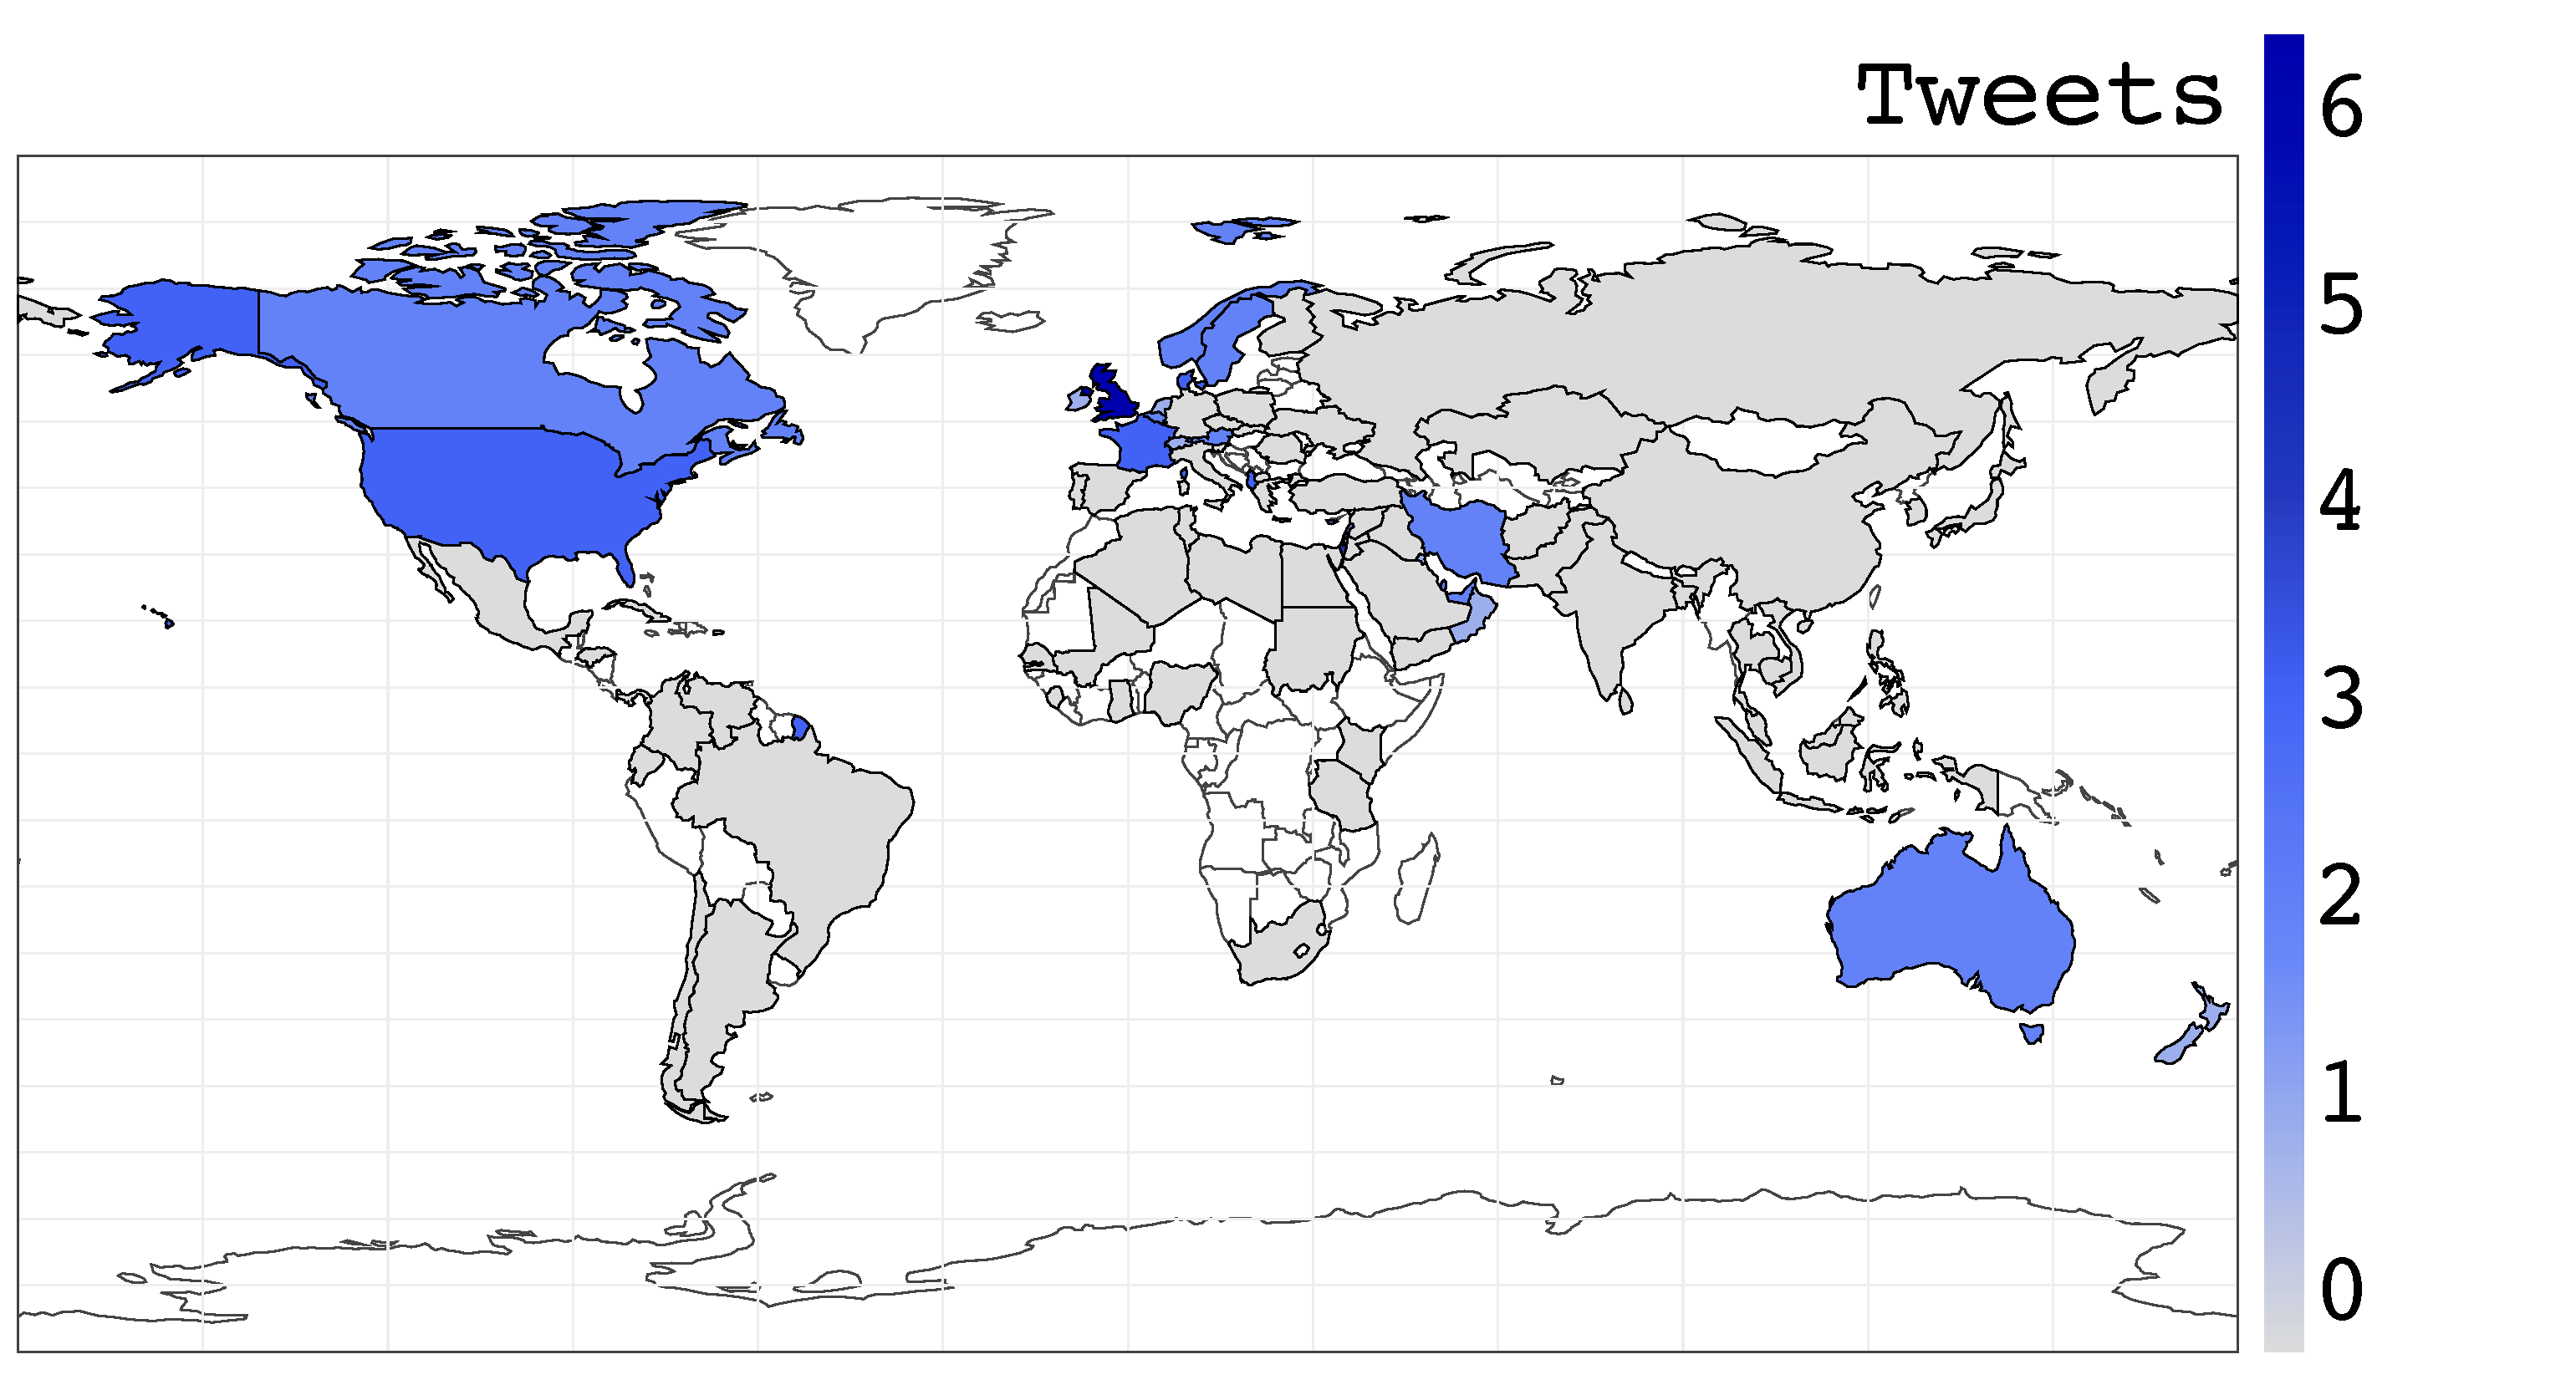
\includegraphics[width=5.3cm]{images/location/world/socialsensor-world-irannucleardeal_location.eps}}
\subfloat[Fig:][Soccer]{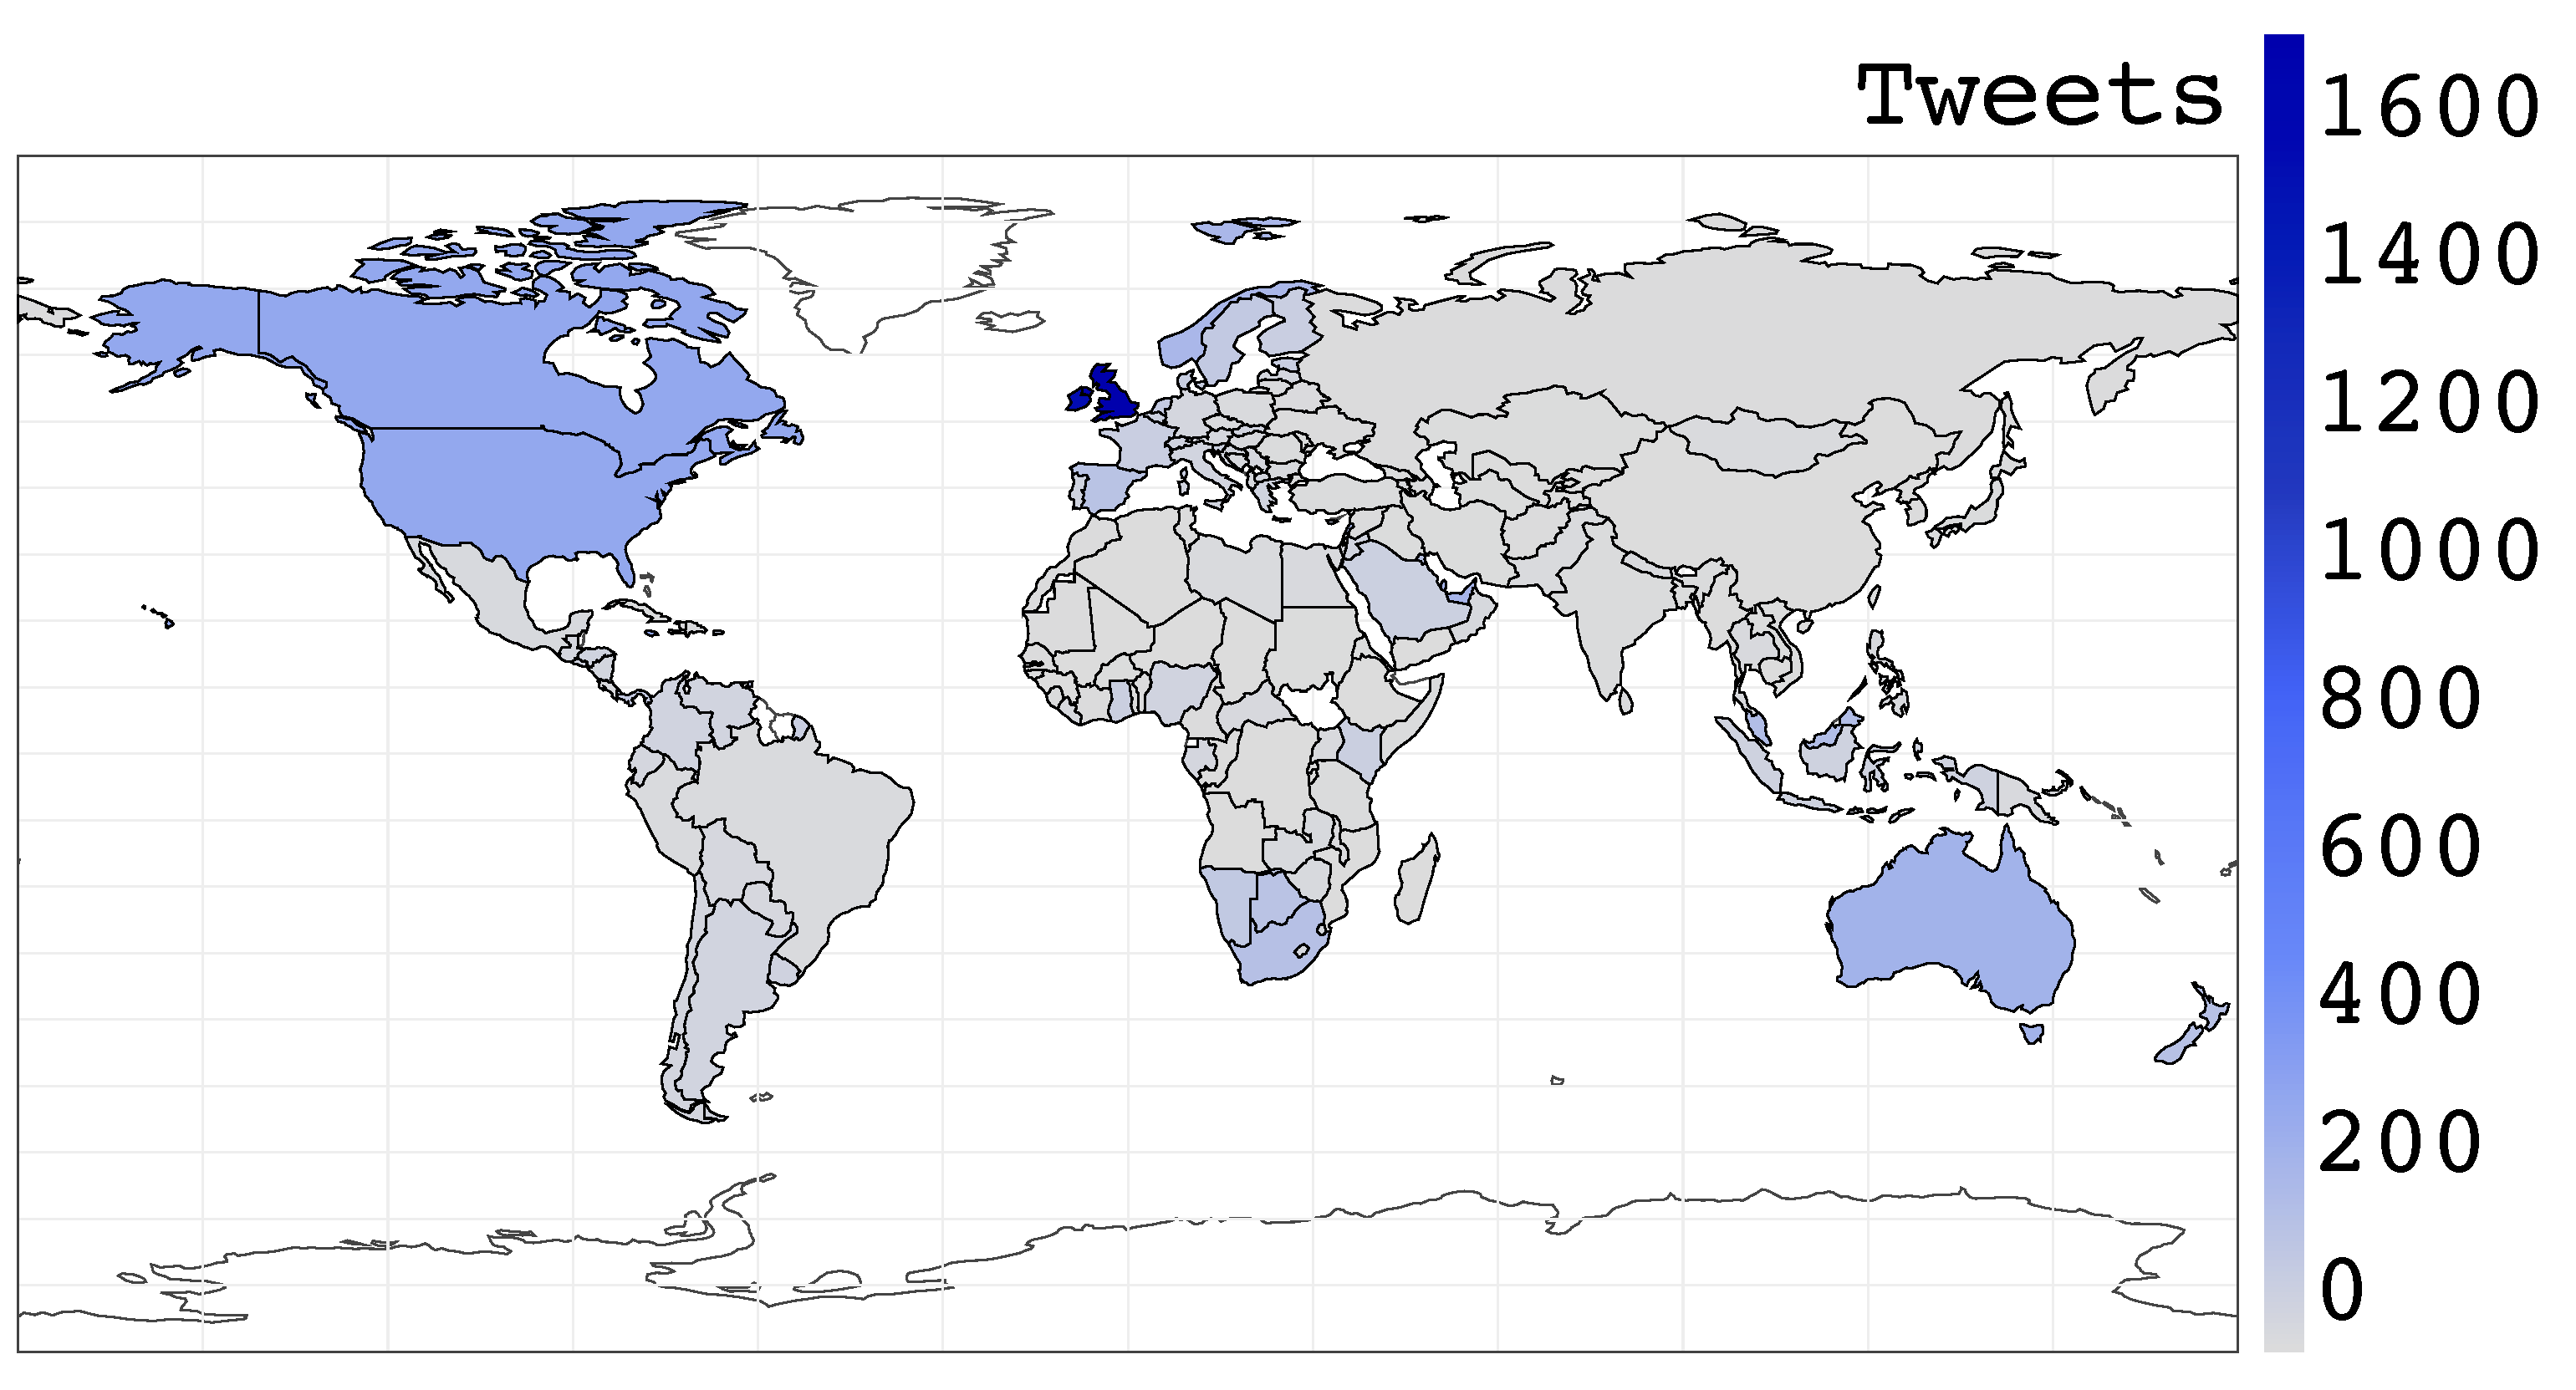
\includegraphics[width=5.3cm]{images/location/world/socialsensor-world-soccer_location.eps}} \\
%\vspace{-10mm}
\subfloat[Fig:][Health Epidemics]{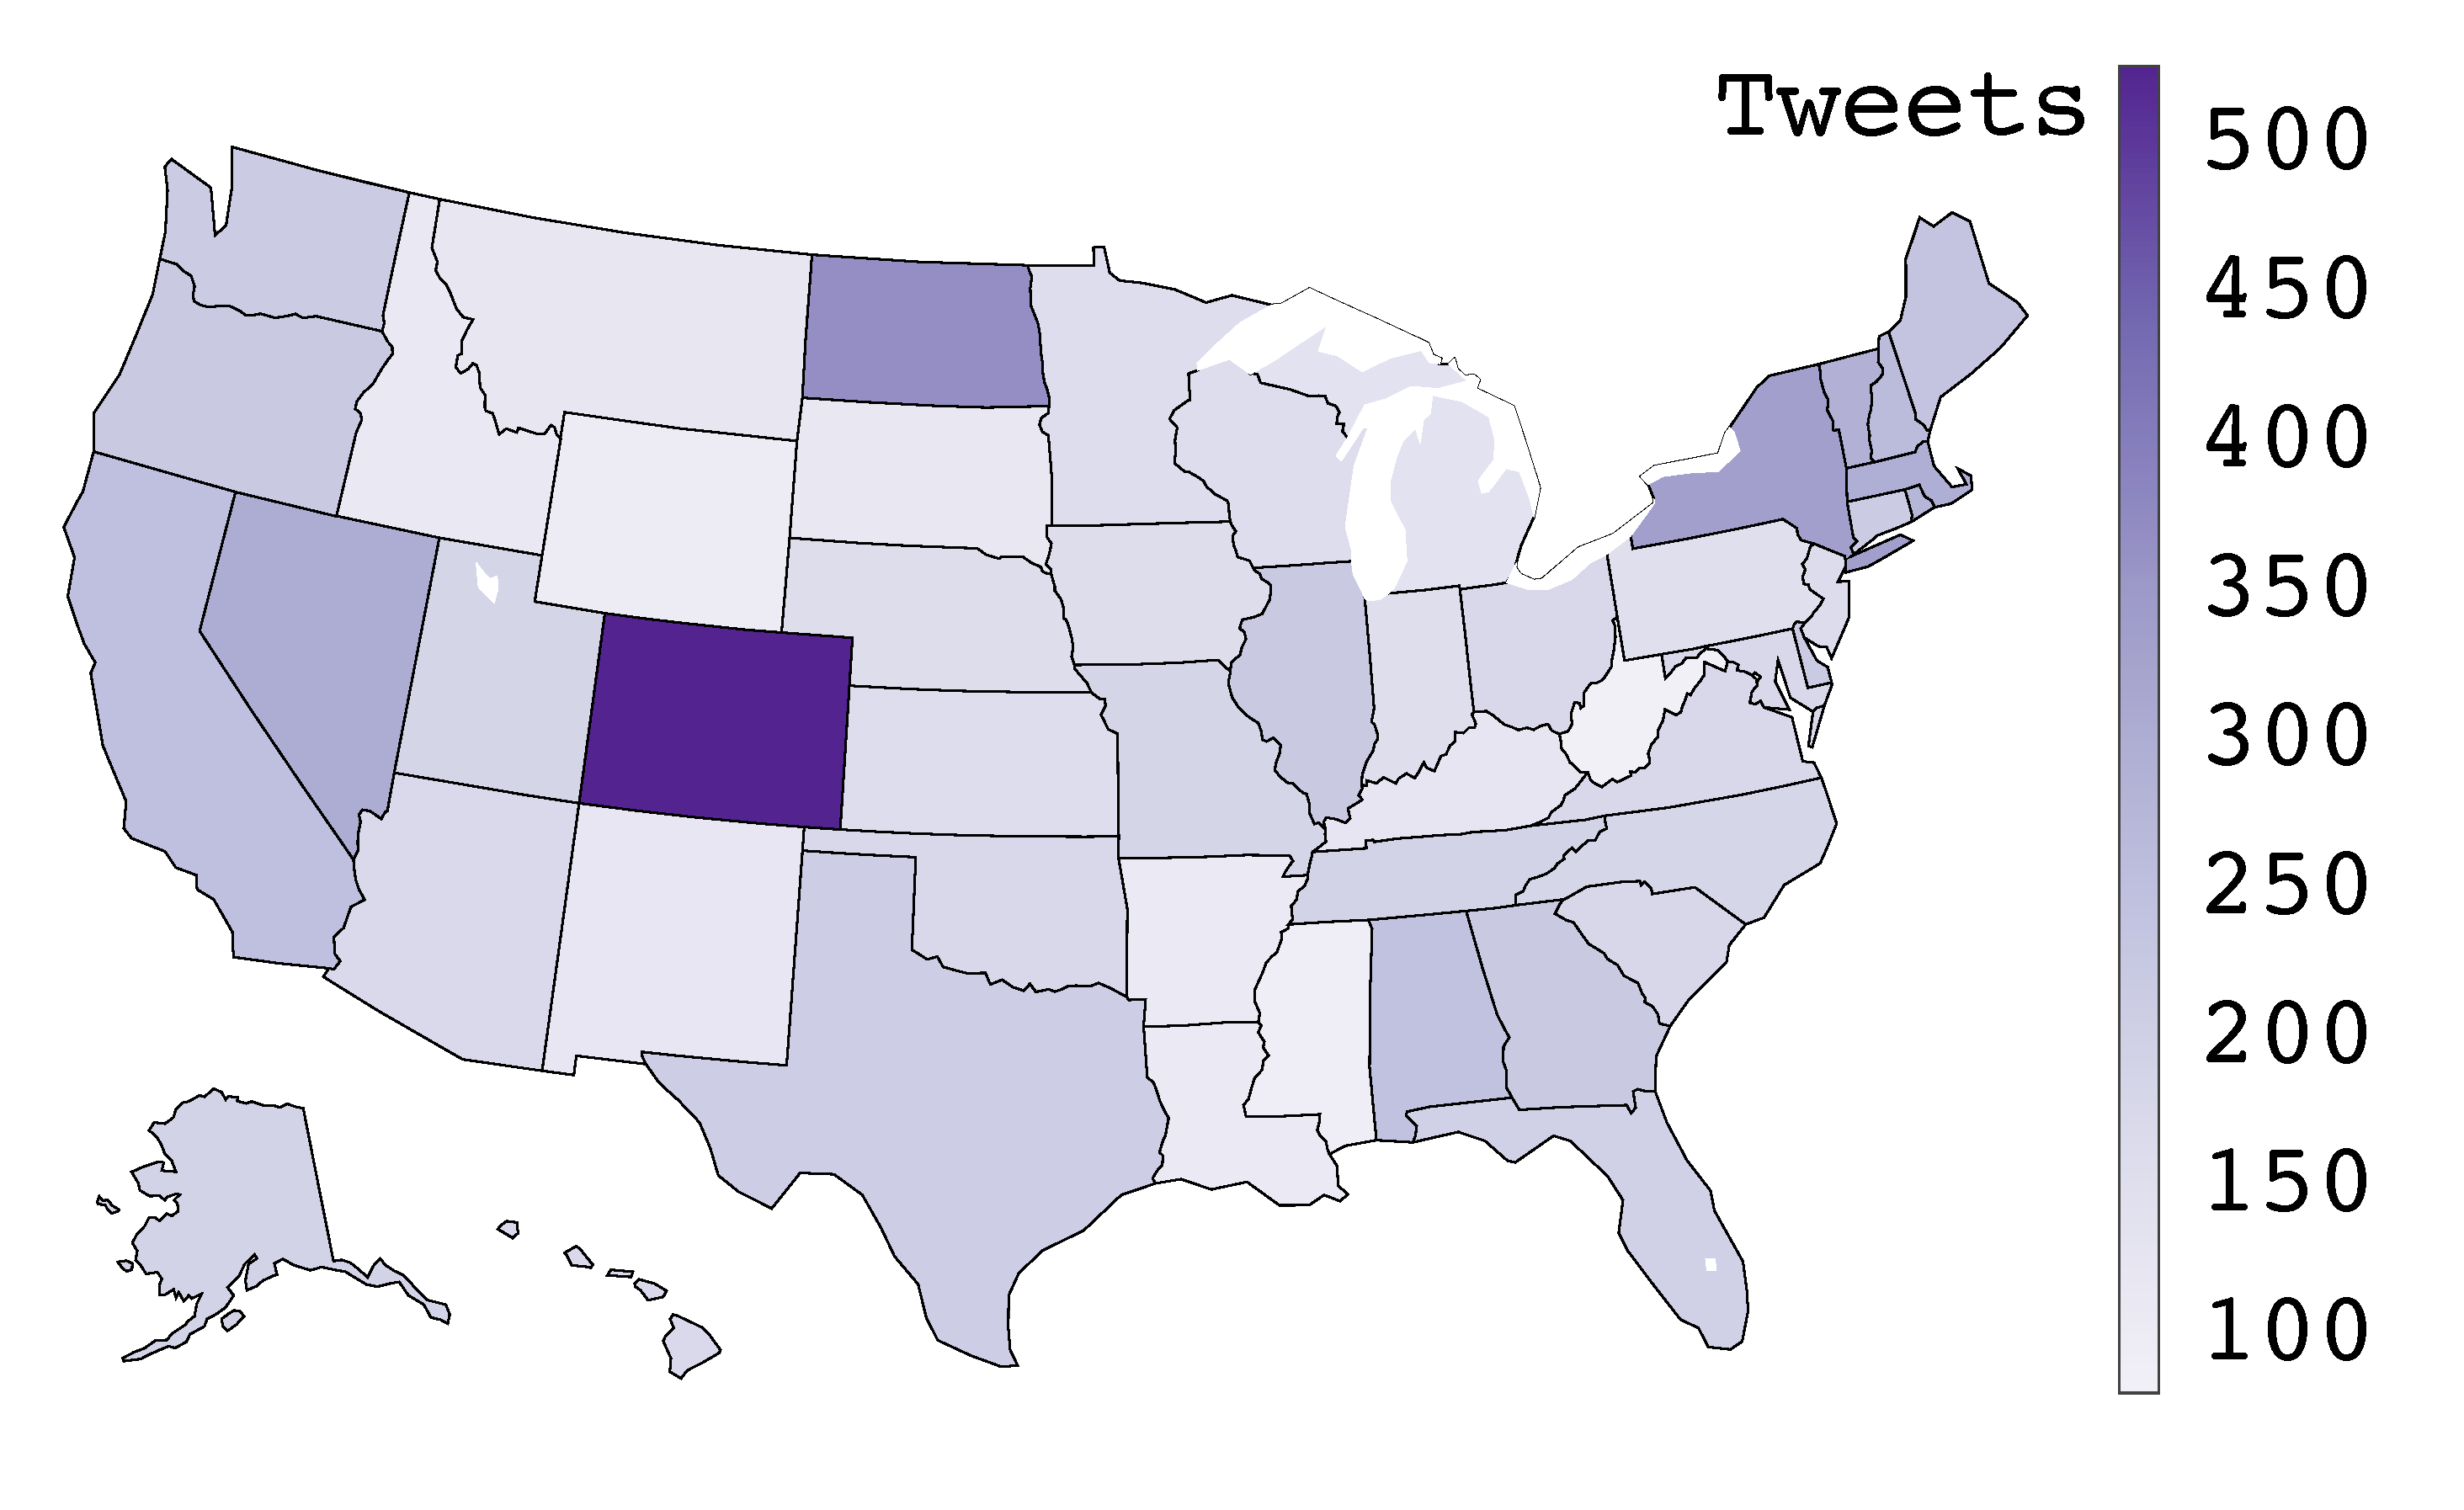
\includegraphics[width=5.3cm]{images/location/states/SocialSensor-us-states-health_epidemics_location.eps}}
\subfloat[Fig:][Social Issues]{\includegraphics[width=5.3cm]{images/location/states/SocialSensor-us-states-socialissues_location.eps}}
\subfloat[Fig:][Space]{\includegraphics[width=5.3cm]{images/location/states/SocialSensor-us-states-space_location}} \\
\end{tabular}
\end{tabular}
\vspace{-2mm}
\caption {Distribution of tweets across International locations (top row) and U.S. locations (bottom row)}
\label{fig:choropleths}
\end{figure*}
%%%%%%%%%%%%%%%%%%%%%%%%%%%%%%%%%%%%%%%%%%%%%%%%%%%%%%%%%%%%%%%%%%%%%%%%%%%

%%%%%%%%%%%%%%%%%%%%%%%%%%%%%%%%%%%%%%%%%%%%%%%%%%%%%%%%%%%%%%%%%%
\begin{table}[th!]
\centering
{\renewcommand{\arraystretch}{1.2}
\resizebox{0.5\textwidth}{!}{%
\begin{tabular}{|l|c|c|c|c|}
\hline
\multicolumn{5}{|c|}{\textbf{Used in \#Tweets}} \\ \hline
\textbf{Feature} & \textbf{Max} & \textbf{Avg} & \textbf{Median} & \textbf{Max entity} \\ \hline
\textbf{From} & 10,196 & 8.67 & 2 & running\_status \\ \hline
\textbf{Hashtag} & 1,653,159 & 13.91 & 1 & \#retweet \\ \hline
\textbf{Mention} &  &  &  &  \\ \hline
\textbf{Location} &  &  &  &  \\ \hline
\textbf{Term} & 241,896,559 & 492.37 & 1 & rt \\ \hline \hline
\multicolumn{5}{|c|}{\textbf{Used by \#Users}} \\ \hline
\textbf{Hashtag} & 592,363 & 10.08 & 1 & \#retweet \\ \hline
\textbf{Mention} & 26,293 & 5.44 & 1 & dimensionist \\ \hline
\textbf{Location} & 739,120 & 641.5 & 2 & london \\ \hline
\textbf{Term} & 1,799,385 & - & 1 & rt \\ \hline \hline
\multicolumn{5}{|c|}{\textbf{Using \#Hashtags}} \\ \hline
\textbf{From} & 18,167 & 2 & 0 & daily\_astrodata \\ \hline
\end{tabular}
}}
\caption{Feature Statistics of $829,026,458$ tweets in our Twitter dataset}
\label{table:featureStatistics}
\end{table}

\begin{table}[th!]
\centering
{\renewcommand{\arraystretch}{1.2}
\resizebox{0.5\textwidth}{!}{%
\begin{tabular}{|l|c|c|c|c|c|}
\hline
 & \textbf{From} & \textbf{Hashtag} & \textbf{Mention} & \textbf{Location} & \textbf{Term} \\ \hline
\textbf{\#Unique} & 95,547,198 & 11,183,410 & 411,341,569 & 58,601 & 20,234,728 \\ \hline
\end{tabular}
}}
\caption{Number of unique values for each feature of $829,026,458$ tweets in our Twitter dataset}
\label{table:featureUnique}
\end{table}
%%%%%%%%%%%%%%%%%%%%%%%%%%%%%%%%%%%%%%%%%%%%%%%%%%%%%%%%%%%%%%%%%%

\section{Empirical Evaluation}
\label{sec:methodology}
How we curated hashtags: need to make up good story here.  Inner-annotator agreement of 3/4.

Train/validation/test split date selection -- temporally .5,.1,.4

Feature selection: threshold per feature 159 and 50 (just explain rationale for lower hashtag and location thresholds).

Formal notation, how do we train/test and tune hyperparameters for a generic classifier.

\subsection{Classification Algorithms}

\begin{enumerate}
\item Naive Bayes
\item Rocchio (centroid)
\item Logistic Regression
\end{enumerate}

All above over 1,000,000 features, *same* training data for all algorithms.

Not breaking down by feature type yet -- that's for the feature analysis section.

\subsection{Analysis}

- Table of rows:alg, cols: MAP, P@k (k in {10,100,1000}) with stderrs over all topics

- Could do a bar graph (below) each for MAP, P@100 with topics as major columns and algs as neighboring bars

- Anecdotal results for each topic -- point out deficiency in our labels (a good thing, we generalized well from small hashtag set), manual evaluation of relevance for top-100 for best algorithm?

%%%%%%%%%%%%%%%%%%%%%%%%%%%%%%%%%%%%%%%%%%%%%%%%%%%%%%%%%%%%%%%%%%
\begin{table*}[t]
\centering
{\renewcommand{\arraystretch}{1.2}
\resizebox{\textwidth}{!}{%
\begin{tabular}{|l|l|c|c|c|c|c|c|c|c|c|c|c|}
\hline
\textbf{Method} & \textbf{Metric} & \textbf{Tennis} & \textbf{Space} & \textbf{Soccer} & \textbf{IranDeal} & \textbf{HumanCausedDisaster} & \textbf{CelebrityDeath} & \textbf{SocialIssues} & \textbf{NaturalDisaster} & \textbf{Epidemics} & \textbf{LGBT} & \textbf{Mean$\pm$Std} \\ \hline
\textbf{LR} & \textbf{MAP} & 0.918 & 0.870 & 0.827 & 0.811 & 0.761 & 0.719 & 0.498 & 0.338 & 0.329 & 0.165 & 0.623$\pm$0.19 \\ \hline
\textbf{NB} & \textbf{MAP} & 0.908 & 0.897 & 0.731 & 0.824 & 0.785 & 0.748 & 0.623 & 0.267 & 0.178 & 0.092 & 0.605$\pm$0.22 \\ \hline
\textbf{Rocchio} & \textbf{MAP} & 0.690 & 0.221 & 0.899 & 0.584 & 0.481 & 0.253 & 0.393 & 0.210 & 0.255 & 0.089 & 0.407$\pm$0.18 \\ \hline
\textbf{RankSVM} & \textbf{MAP} & 0.702 & 0.840 & 0.674 & 0.586 & 0.603 & 0.469 & 0.370 & 0.248 & 0.136 & 0.082 & 0.471$\pm$0.18 \\ \hline \hline
\textbf{LR} & \textbf{P@10} & 1.000 & 0.000 & 0.200 & 0.700 & 0.600 & 0.000 & 0.100 & 0.200 & 0.300 & 0.500 & 0.360$\pm$0.24 \\ \hline
\textbf{NB} & \textbf{P@10} & 1.000 & 0.900 & 0.700 & 0.600 & 0.600 & 0.700 & 1.000 & 0.100 & 0.400 & 0.100 & 0.610$\pm$0.23 \\ \hline
\textbf{Rocchio} & \textbf{P@10} & 0.800 & 0.000 & 1.000 & 0.900 & 0.000 & 0.000 & 0.000 & 0.500 & 0.500 & 0.100 & 0.380$\pm$0.29 \\ \hline
\textbf{RankSVM} & \textbf{P@10} & 1.000 & 0.800 & 0.600 & 0.800 & 0.400 & 0.300 & 0.000 & 0.100 & 0.000 & 0.200 & 0.420$\pm$0.26 \\ \hline \hline
\textbf{LR} & \textbf{P@100} & 0.950 & 0.580 & 0.650 & 0.870 & 0.620 & 0.490 & 0.640 & 0.690 & 0.790 & 0.210 & 0.649$\pm$0.15 \\ \hline
\textbf{NB} & \textbf{P@100} & 0.980 & 0.850 & 0.600 & 0.880 & 0.750 & 0.860 & 0.730 & 0.230 & 0.090 & 0.190 & 0.616$\pm$0.23 \\ \hline
\textbf{Rocchio} & \textbf{P@100} & 0.980 & 0.000 & 1.000 & 0.690 & 0.170 & 0.000 & 0.280 & 0.170 & 0.680 & 0.120 & 0.409$\pm$0.28 \\ \hline
\textbf{RankSVM} & \textbf{P@100} & 0.730 & 0.720 & 0.310 & 0.700 & 0.880 & 0.440 & 0.480 & 0.340 & 0.020 & 0.100 & 0.472$\pm$0.20 \\ \hline \hline
\textbf{LR} & \textbf{P@1000} & 0.963 & 0.954 & 0.816 & 0.218 & 0.899 & 0.833 & 0.215 & 0.192 & 0.343 & 0.071 & 0.550$\pm$0.26 \\ \hline
\textbf{NB} & \textbf{P@1000} & 0.954 & 0.954 & 0.716 & 0.218 & 0.904 & 0.881 & 0.215 & 0.195 & 0.141 & 0.060 & 0.524$\pm$0.28 \\ \hline
\textbf{Rocchio} & \textbf{P@1000} & 0.604 & 0.000 & 0.925 & 0.218 & 0.359 & 0.000 & 0.215 & 0.167 & 0.144 & 0.065 & 0.270$\pm$0.21 \\ \hline
\textbf{RankSVM} & \textbf{P@1000} & 0.799 & 0.922 & 0.764 & 0.218 & 0.525 & 0.547 & 0.215 & 0.173 & 0.154 & 0.064 & 0.438$\pm$0.22 \\ \hline
\end{tabular}
}}
\caption{Different learning methods results on topics with hyper-parameter tuning based on MAP}
\label{table:results2}
\end{table*}
%%%%%%%%%%%%%%%%%%%%%%%%%%%%%%%%%%%%%%%%%%%%%%%%%%%%%%%%%%%%%%%%%%

%%%%%%%%%%%%%%%%%%%%%%%%%%%%%%%%%%%%%%%%%%%%%%%%%%%%%%%%%%%%%%%%%%
\begin{table*}[]
\large
{\renewcommand{\arraystretch}{1.2}
\resizebox{\textwidth}{!}{
\begin{tabular}{|l|l|}
\hline
\textbf{Tennis} & \textbf{Space} \\ \hline 
\checkmark rt @espntennis: shock city. darcis drops rafa in straight sets. first time nadal loses in first rd of a. major in career. \#espnwimbledon \#wÉ & \xmark  rt @jaredleto: rt @30secondstomars: icymi: mars performing a cover of @rihanna's \#stay on australia's @triplemmelb - video \_ http://t.co/uqÉ \\ \hline
\checkmark rt @espntennis: shock city. darcis drops rafa in straight sets. first time nadal loses in first rd of a. major in career. \#espnwimbledon \#wÉ & \xmark  voting mars @30secondstomars @jaredleto @shannonleto @tomofromearth xobest group http://t.co/dlsozvjinf \\ \hline
\checkmark rt @espntennis: shock city. darcis drops rafa in straight sets. first time nadal loses in first rd of a. major in career. \#espnwimbledon \#wÉ & \xmark  rt @jaredleto\_com: show everyone how much you are proud of @30secondstomars !\#mtvhottest 30 seconds to mars http://t.co/byxnri4t67 \\ \hline
\checkmark rt @espntennis: shock city. darcis drops rafa in straight sets. first time nadal loses in first rd of a. major in career. \#espnwimbledon \#wÉ & \xmark  rt @30secondstomars: missed the big news? mars touring with @linkinpark + special guests @afi this summer!\_ http://t.co/3e5rm9pwrd \\ \hline
\checkmark rt @espntennis: shock city. darcis drops rafa in straight sets. first time nadal loses in first rd of a. major in career. \#espnwimbledon \#wÉ & \xmark  rt @30secondstomars: to the right,to the left,we will fightto the death.go \#intothewildonvyrt with mars, starting weekly, nov 30 \_ httÉ \\ \hline
\textbf{Soccer} & \textbf{IranDeal} \\ \hline
\xmark  rt @tomm\_dogg: \#thingstodobeforeearthends spend all my money. & \checkmark rt @iran\_policy: @vidalquadras:@isjcommittee has investigated 10 major subjects of iranŐs controversial \#nuclear program \#irantalksvienna \\ \hline
\starmark  @mancityonlineco nice performance & \checkmark rt @iran\_policy: @vidalquadras:@isjcommittee has investigated 10 major subjects of iranŐs controversial \#nuclear program \#irantalksvienna \\ \hline
\starmark  rt @indykaila: podolski: "let's see what happens in the winter. the fact is that i'm not happy with it, that's clear." @arsenal & \xmark  rt @negarmortazavi: thank you @hassanrouhani for retweeting. let's hope for a day when no iranian fears returning to their homeland. http:/É \\ \hline
\starmark  rt @indykaila: wenger: "i don't believe match-fixing is a problem in england." \#afc & \xmark  rt @iran\_policy: iran: details of savage attack on political prisoners in evin prison http://t.co/xdzuakqdiv \#iran \#humanrights \\ \hline
\xmark  @indykaila you never got back to me about tennis this week & \checkmark rt @iran\_policy: chairman ros-lehtinen speaking on us commitment 2 protect camp liberty residents. \#iranhrviolations http://t.co/1g6dhx1znu \\ \hline
\textbf{HumanCausedDisaster} & \textbf{CelebrityDeath} \\ \hline
\checkmark rt @baselsyrian: there`ve been peaceful people in \#homs not terrorists! \#assad,enemy of \#humanity destroyed it. \#eyeonhoms \#withsyria http:É & \starmark  rt @sawubona\_chris: today is my birthday \&amp; also the day my hero @nelsonmandela has died. lets never forget what he taught us. forgiveness iÉ \\ \hline
\checkmark what a helpless father, he can do nothing under \#assad's siege!\#speakup4syrianchildren  http://t.co/vgle3byebw\#syria \#syriawarcrimes \#un & \starmark  rt @nelsonmandela: Ňdeath is something inevitable.when a man has done what he considers to be his duty to his people\&amp;his country,he can resÉ \\ \hline
\starmark  exclusive: us formally requested \#un investigation; russia pressured \#assad to no avail;chain of evidence proof hard http://t.co/560t2rvdfw & \starmark  rt @nelsonmandela: la muerte es algo inevitable.cuando un hombre ha hecho lo que considera que es su deber para con su gente y su pa’s,puedÉ \\ \hline
\starmark  \#save\_aleppo from \#assadwarcrimes\#save\_aleppo from \#civilians -targeted shelling of \#assad regime\#syria \#aleppo http://t.co/k3dfxh0pxl & \xmark   \#jacques \#kallis: a phenomenal cricketing giant of all time - \#cricket \#history \#southafrica http://t.co/ms5pmwoag9 \\ \hline
\checkmark rt @canine\_rights: why does the \#un allow this to continue? rt@tintin1957 help raise awareness of the suffering in \#syriawarcrimes http://tÉ & \xmark  @sudesh1304 south africa has the most beautiful babies....so diverse,so unique...so god!! lol \#durban \#southafrica \\ \hline
\textbf{SociallIssues} & \textbf{NaturalDisaster} \\ \hline
\starmark  the us doesn't actually borrow is the thing. i believe in a creationist theory of the us dollar @usanationdebt @nationaldebt & \xmark  us execution in \#oklahoma :  not cruel and unusual?  maybe just barbaric, inhumane and reminiscent of the dark ages! \\ \hline
\starmark  rt @2anow: according to @njsenatepres women's rights do not include this poor nj mother's right to defend herself http://t.co/xzbslnqkh6  \#É & \xmark  \#haiti \#politics - the haiti-dominican crisis - i agree with how martelly is handling the situation: i totally... http://t.co/ro4pswsszs \\ \hline
\starmark  rt @2anow: confiscation ? how many carry permits are in the senate and assembly? give us ours or turn them in.  @senatorlorettaw @lougreenwÉ & \starmark  rt @soilhaiti: a new reforestation effort in \#haiti. local compost, anyone? http://t.co/xpad0rqbjk @richardbranson @clintonfdn @virginuniteÉ \\ \hline
\starmark  rt @2anow: vote with your wallet against \#guncontrolforest city enterprises does not support the \#2a http://t.co/tpkok3berm\#nj2as  \#tcot & \xmark  mes cousins jamais nŽs hantent les nuits de duvalier \#haiti \#duvalier \\ \hline
\starmark  @2anow @momsdemand @jstines3 they dont have a plan for that , which is why they should never be allowed to take our guns & \checkmark tony burgener of @swisssolidarity says you can't compare the disaster response in \#haiti with the response to \#haiyan in \#philippines @iheid \\ \hline
\textbf{Epidemics} & \textbf{LGBT} \\ \hline
\checkmark rt @who: fourteen of the susp. \&amp; conf. ebola cases in \#conakry, \#guinea, are health care workers, of which 11 died \#askebola & \starmark  rt @jackmcoldcuts: @lunaticrex @fingersmalloy @toddkincannon @theanonliberal anthony kennedy just wrote opinion granting legal protection to cupcake kiplers \\ \hline
\xmark  @who who can afford also been cover in government health insurance {[}with universal health coverage{]} & \xmark  @toddkincannon your personal account, your interest. separate from your business. \\ \hline
\checkmark \#ebolaoutbreak this health crisis..unparalleled in modern times,Ó @who dir. aylward - requires \$1 billion to stem http://t.co/rjzqhydb3d & \xmark  why would you report someone as spam if he is not spam? @illygirlbrea @toddkincannon \\ \hline
\xmark  rt @medsin: @who are conducting a survey on the social determinants of health in medical teaching. fill the survey in at https://t.co/aj59xÉ & \xmark  rt @t3h\_arch3r: @toddkincannon thanks for your tl having the female realbrother. between them is 600 lbs. 104 iq points. and a lot of hate. \\ \hline
\xmark  augmentation vertigineuse de 57,4\% en 1 an des actes islamophobes en france, dit le collectif contre l'islamophobie http://t.co/2qjhocegi5 & \xmark  @toddkincannon who us dick trickle. \\ \hline
\end{tabular}
}
}
\caption{Top Tweets for each topic based on MAP tuned results}
\label{table:topTweets}
\end{table*}
%%%%%%%%%%%%%%%%%%%%%%%%%%%%%%%%%%%%%%%%%%%%%%%%%%%%%%%%%%%%%%%%%%


\section{Feature Analysis}
\label{label:featureanalysis}.
%\textbf{What we have to work with: topics, features, feature attributes}
In this section, we analyze the informativeness of each feature for learning topical tweets by looking at different characteristics for each feature in our dataset. For example, one characteristic of hashtags could be the number of the tweets that contain those hashtags. Does this have an effect on importance of the hashtag when it comes to learning topical tweets or not. In this sense, this section would bring insights to the following questions:

\begin{itemize}
\item \textbf{What are the best features for learning social sensors, do they differ by topic?  (Why?)}
\item \textbf{For each feature type, do any attributes correlate with importance?}
\end{itemize}

A famous method for measuring informativeness is Mutual Information which is a measure of amount of information one random variable contains about another random variable. In order to calculate amount of information that a feature $f_k \in \{from, hashtag, mention, term, location\}$ provides w.r.t $t_i \in \{NaturalDisaster, Epidemics, ...\}$, mutual information is defined as:

\begin{multline}
I(t_i, f_k)= \\
 \sum_{t_i\in \{ true, false \}} \sum_{f_k\in \{ true, false\}}p(f_k,t_i)\log \left ( \frac{p(f_k,t_i)}{p(f_k)p(t_i)} \right )
 \label{eq:eq1}
\end{multline}

Higher values for this metric indicates more informative features for the specified topic.

First, we provide mutual information values for each feature across different topics shown by boxplots in figure \ref{fig:miboxplots}, and average values of mutual information for each feature vs different topics shown in table \ref{fig:table1}. The last column in table \ref{fig:table1} shows average mutual information for the feature with the standard error range provided. We make a few observations from the analysis of Table \ref{fig:table1}:

\begin{itemize}
\item Term features provide more information for all of the topics on average which shows the importance of uni-grams when it comes to selection of topical tweet.
\item From and mention features are the least informative features for all of the topics.
\item Location and Hashtag feature provide second and third most informative features respectively.
\item A few topics such as irandeal and tennis are less sensitive to selection of a specific features.
\item Location feature provides more information regarding HumanDisaster, LBGT, and Soccer topics.
\item Sorting features based on their average mean value across different topics results in the following order:
\begin{enumerate}
\item Term
\item Location
\item Hashtag
\item Mention
\item From
\end{enumerate}
\end{itemize}

%%%%%%%%%%%%%%%%%%%%%%%%%%%%%%%%%%%%%%%%%%%%%%%%%%%%%%%%%%%%%%%%%%%%%%%%%%%
\iffalse
\begin{figure}[tbph!]
\centering
\includegraphics[width=0.5\textwidth]{images/avgMI.pdf}
\vspace{-3mm}
\caption{Average MI for different features vs. Topics, last two column show mean value and stderr across all topics}
\label{fig:table1}
\end{figure}
\fi
\begin{figure}[h!]
\centering
\includegraphics[width=0.5\textwidth]{images/medianMI.pdf}
\vspace{-3mm}
\caption{Median MI for different features vs. Topics, last two column show mean value and stderr across all topics}
\label{fig:table1}
\end{figure}
\
\begin{figure}[h!]
\centering
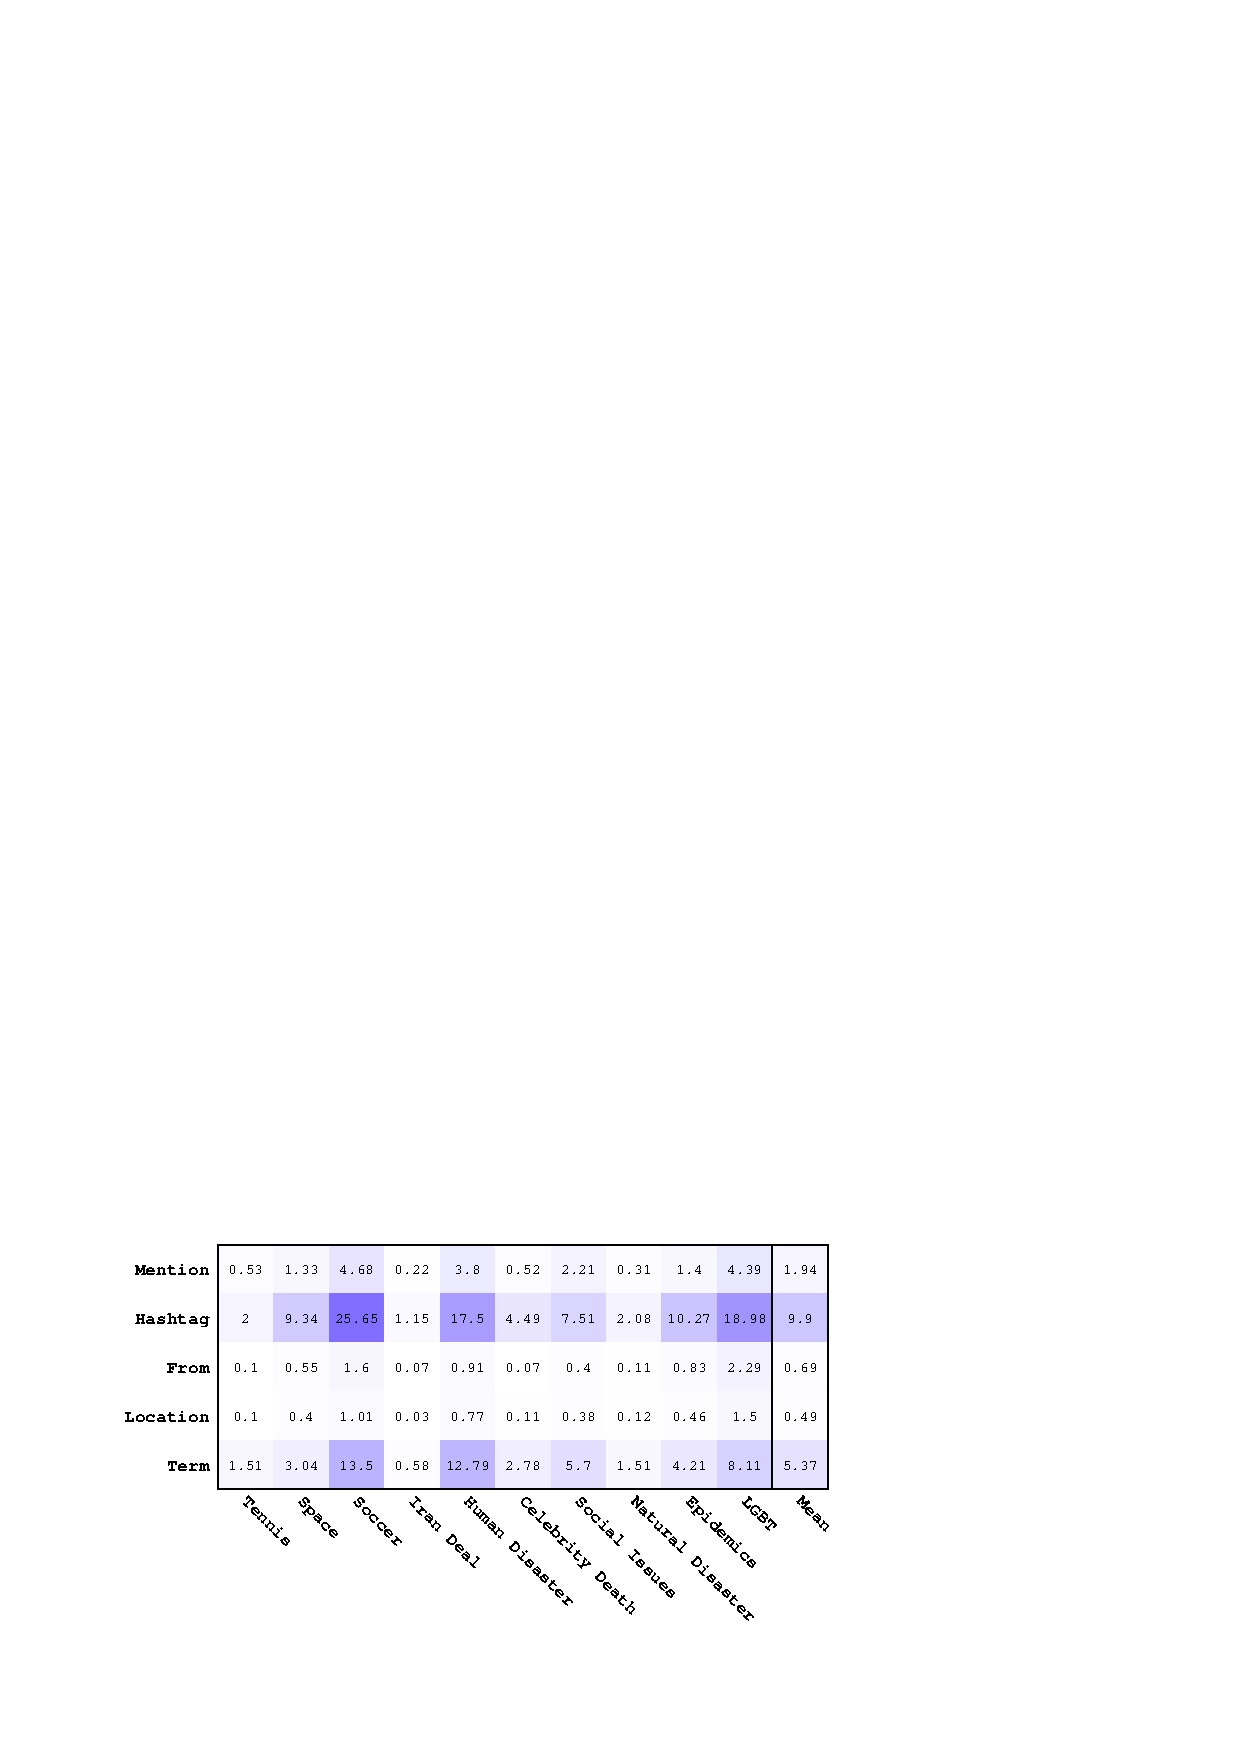
\includegraphics[width=0.5\textwidth]{images/avgMI_gray.pdf}
\vspace{-3mm}
\caption{Average MI for different features vs. Topics, last two column show mean value and stderr across all topics}
\label{fig:table1}
\end{figure}
%%%%%%%%%%%%%%%%%%%%%%%%%%%%%%%%%%%%%%%%%%%%%%%%%%%%%%%%%%%%%%%%%%%%%%%%%%%

It is important to note that due to very large amount of Term features, they were cleaned based on their frequency (having at least frequency value of 100).

\textbf{For each feature type, do any attributes correlate with importance?} In order to give a better sense of what features are better for each topic, we provided top-5 features for each topic in table \ref{table:top10MItopicsLocations}. It can be observed how different locations, hashtags, or terms showed as the top features based on mutual information are actually in relation with the specific topic.%\begin{enumerate}
%\color{red}
%\item Anecdotal feature analysis: for each of 5 feature types: (rows) top-k / median-k (?), (cols) topics -- much better than below b/c we show all topics here and we can compare features across topics.
%Don't use for now: show (rows) top-k and median-k features for different topics and (cols) 5 features (location, mention, from, term, hashtag) -- need to select a **few (2-3) interesting topics** and explain shown in table \ref{top10MItopicsLocations}
%\end{enumerate}

%%%%%%%%%%%%%%%%%%%%%%%%%%%%%%%%%%%%%%%%%%%%%%%%%%%%%%%%%%%%%%%%%%
\begin{table*}[ht]
\centering
{\renewcommand{\arraystretch}{1.2}
\resizebox{\textwidth}{!}{%
\begin{tabular}{|l|l|l|l|l|l|l|l|l|l|l|}
\hline
\textbf{Topics/Top10} & \textbf{NaturalDisaster} & \textbf{Epidemics} & \textbf{IranDeal} & \textbf{SocialIssues} & \textbf{LBGT} & \textbf{HumanDisaster} & \textbf{CelebrityDeath} & \textbf{Space} & \textbf{Tennis} & \textbf{Soccer} \\ \hline
\textbf{From} & earthquake\_wo & changedecopine & mazandara & nsingerdebtpaid & eph4\_15 & ydumozyf & nmandelaquotes & daily\_astrodata & tracktennisnews & losangelessrh \\ \hline
\textbf{From} & earthalerts & drdaveanddee & hhadi119 & debtadvisoruk & mgdauber & syriatweeten & boiknox & freesolarleads & tennis\_result & shoetale \\ \hline
\textbf{From} & seelites & joinmentornetwk & 140iran & debt\_protect & stevendickinson & tintin1957 & jacanews & houston\_\_jobs & i\_roger\_federer & sport\_\_agent \\ \hline
\textbf{From} & globalfloodnews & followebola & setarehgan & negativeequityf & lileensvf1 & sirajsol & ewnreporter & star\_wars\_gifts & tennislessonnow & books\_you\_want \\ \hline
\textbf{From} & gcmcdrought & localnursejobs & akhgarshabaneh & dolphin\_ls & truckerbooman & rt3syria & paulretweet & lenautilus & kamranisbest & makeupbella \\ \hline \hline
\textbf{Hashtag} & earthquake & health & iran & ferguson & tcot & syria & rip & science & wimbledon & lfc \\ \hline
\textbf{Hashtag} & haiyan & uniteblue & irantalks & mikebrown & p2 & gaza & riprobinwilliams & starwars & usopen & worldcup \\ \hline
\textbf{Hashtag} & storm & ebola & rouhani & ericgarner & pjnet & isis & ripcorymonteith & houston & tennis & arsenal \\ \hline
\textbf{Hashtag} & tornado & healthcare & iranian & blacklivesmatter & uniteblue & israel & mandela & sun & nadal & worldcup2014 \\ \hline
\textbf{Hashtag} & prayforthephilippines & depression & no2rouhani & fergusondecision & teaparty & mh370 & nelsonmandela & sxsw & wimbledon2014 & halamadrid \\ \hline \hline
\textbf{Location} & philippines & usa & tehran & st.louis & usa & malaysia & southafrica & germany & london & liverpool \\ \hline
\textbf{Location} & ca & ncusa & u.s.a & mo & bordentown & palestine & johannesburg & roodepoort & uk & manchester \\ \hline
\textbf{Location} & india & garlandtx & nederland & usa & newjersey & syria & capetown & houston & india & london \\ \hline
\textbf{Location} & newdelhi & oh-sandiego & iran & dc & sweethomealabama! & israel & pretoria & austin & pakistan & nigeria \\ \hline
\textbf{Location} & newzealand & washington & globalcitizen & washington & aurora & london & durban & tx & islamabad & india \\ \hline \hline
\textbf{Mention} & oxfamgb & foxtramedia & 4freedominiran & deray & jjauthor & ifalasteen & nelsonmandela & bizarro\_chile & wimbledon & lfc \\ \hline
\textbf{Mention} & weatherchannel & obi\_obadike & iran\_policy & natedrug & 2anow & revolutionsyria & realpaulwalker & nasa & usopen & arsenal \\ \hline
\textbf{Mention} & redcross & who & hassanrouhani & antoniofrench & govchristie & drbasselabuward & robinwilliams & j\_ksen & andy\_murray & realmadriden \\ \hline
\textbf{Mention} & twcbreaking & obadike1 & un & bipartisanism & a5h0ka & mogaza & rememberrobin & jaredleto & serenawilliams & ussoccer \\ \hline
\textbf{Mention} & abc7 & c25kfree & statedept & theanonmessage & barackobama & palestinianism & tweetlikegiris & 30secondstomars & espntennis & mcfc \\ \hline \hline
\textbf{Term} & philippines & health & iran & police & obama & israel & robin & cnblue & murray & madrid \\ \hline
\textbf{Term} & donate & ebola & regime & protesters & gun & gaza & williams & movistar & tennis & goal \\ \hline
\textbf{Term} & typhoon & acrx & nuclear & officer & rights & israeli & nelson & enero & federer & cup \\ \hline
\textbf{Term} & affected & medical & iranian & protest & america & killed & mandela & ΍imperdible & djokovic & manchester \\ \hline
\textbf{Term} & relief & virus & resistance & cops & gop & children & cory & greet & nadal & match \\ \hline
\end{tabular}
}}
\caption{Top 5 features for each topic based on Mutual Information}
\label{table:top10MItopicsLocations}
\end{table*}
%%%%%%%%%%%%%%%%%%%%%%%%%%%%%%%%%%%%%%%%%%%%%%%%%%%%%%%%%%%%%%%%%%

\textcolor{red}{
\textbf{\color{red}scatterplots of feature MI -- the absolute last thing we do (density plots?!!)}
**which plots below, and for which topics?  Could pick out most useful features for topics in part (a)(i) and just show selected scatter plots below for these feature types.
from, mention MIs vs. {followers, favorites, friends, hashtags, tweets}
hashtag MI vs. {\#tweets, \#users}
location MI vs. {\#users}
term MI vs. {\#tweets}
}

%%%%%%%%%%%%%%%%%%%%%%%%%%%%%%%%%%%%%%%%%%%%%%%%%%%%%%%%%%%%%%%%%%%%%%%%%%%
\iffalse
\begin{figure*}[tbph!]
\centering
\begin{tabular}{ccccc}
\begin{tabular}{ccccc}
\subfloat[Fig:][Favorite Count]{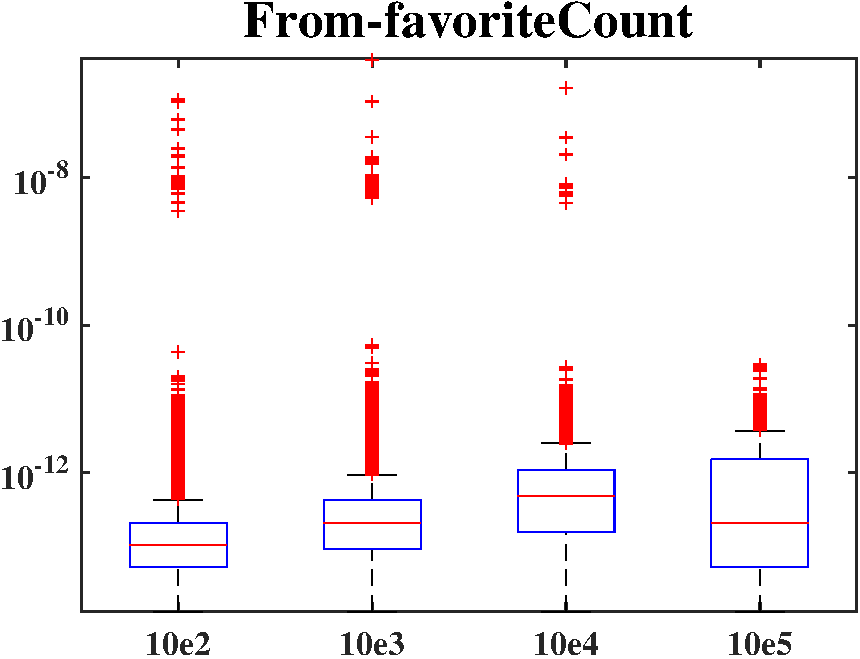
\includegraphics[width=32mm, height=35mm]{images/BoxPlots_IranDeal/From-favoriteCount.pdf}}
\subfloat[Fig:][Followers Count]{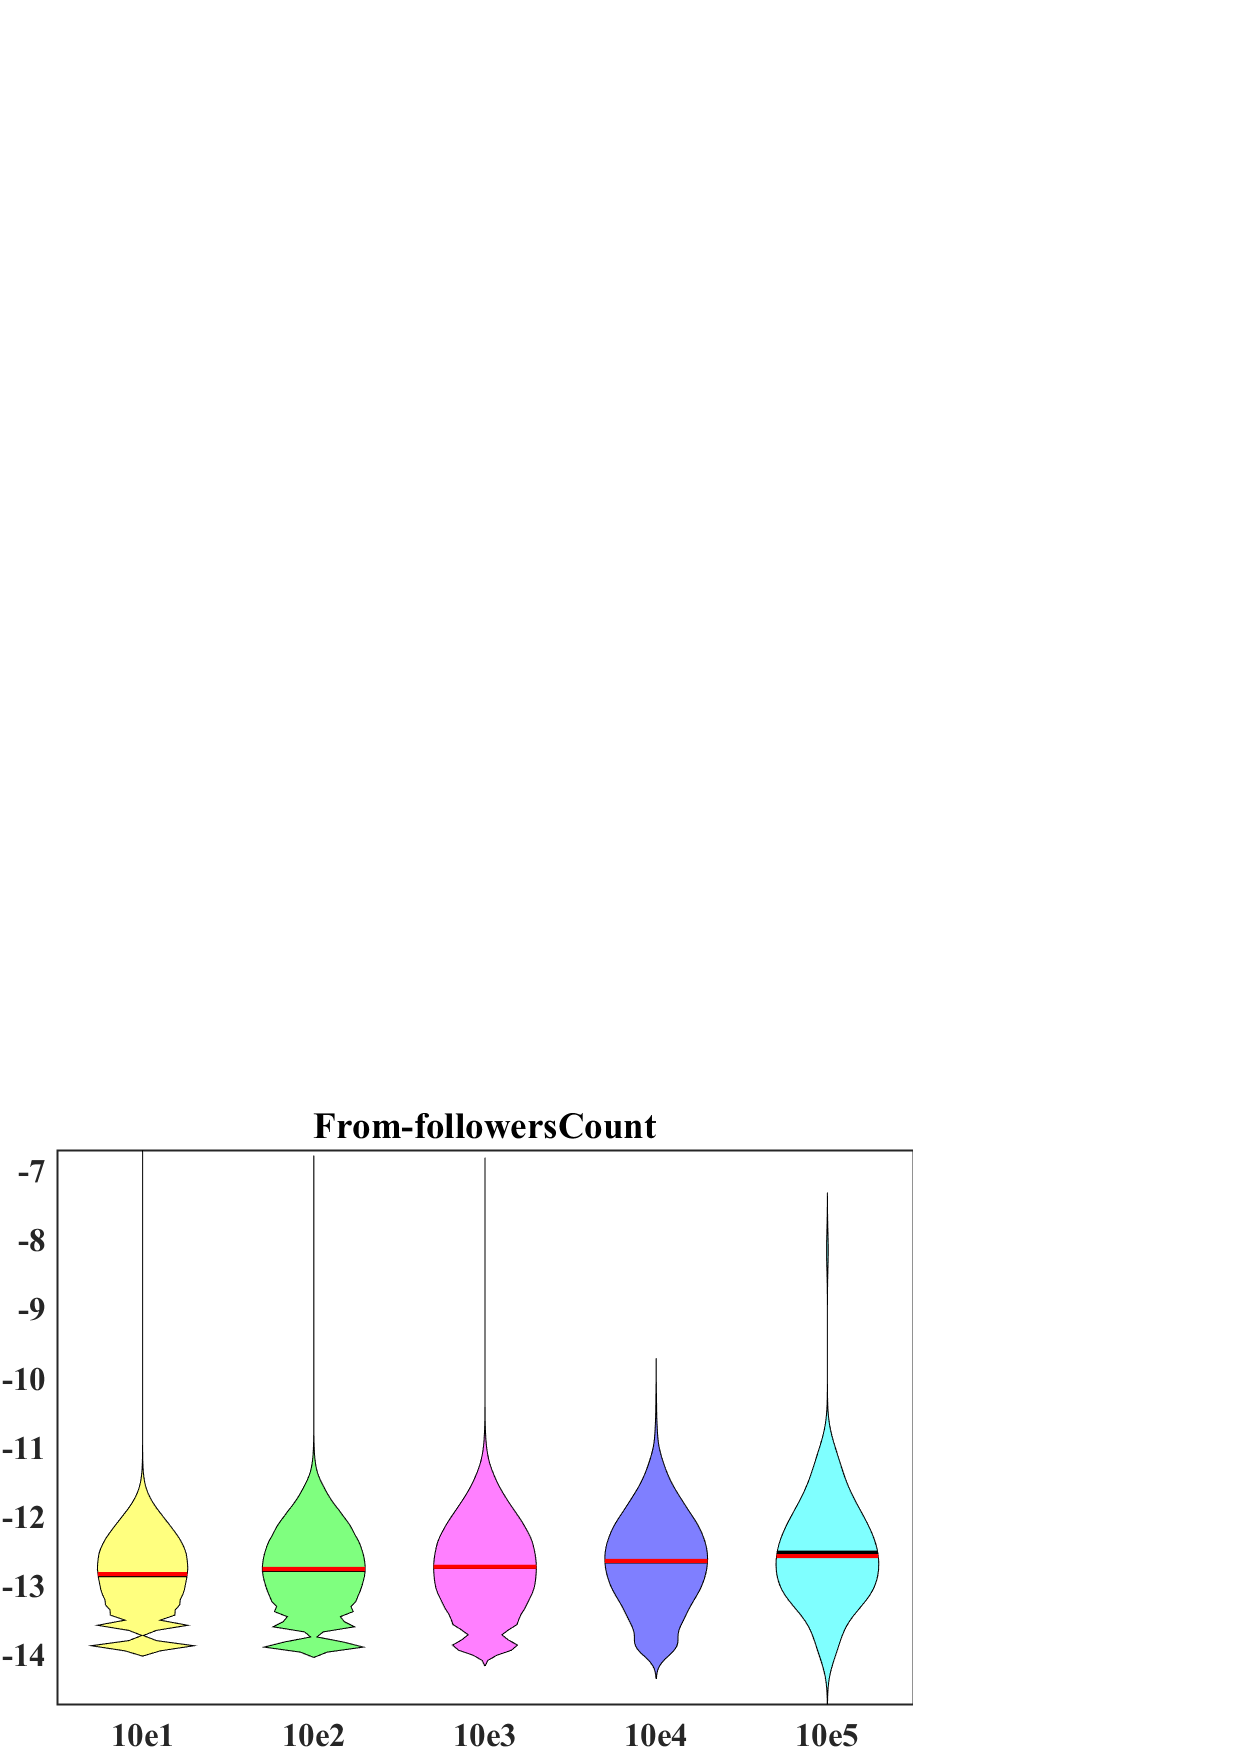
\includegraphics[width=32mm, height=35mm]{images/BoxPlots_IranDeal/From-followersCount.pdf}}
\subfloat[Fig:][Friends Count]{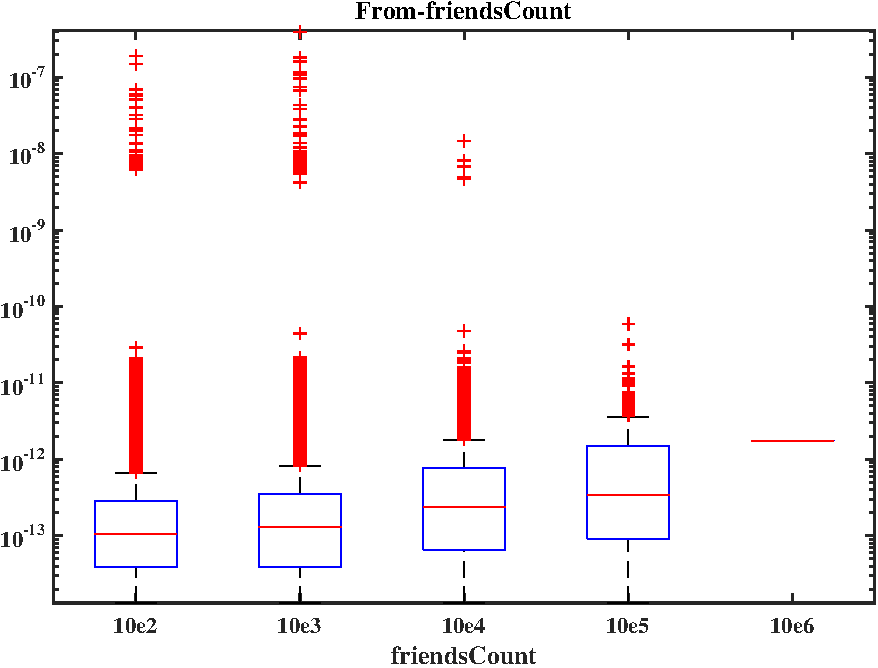
\includegraphics[width=32mm, height=35mm]{images/BoxPlots_IranDeal/From-friendsCount.pdf}}
\subfloat[Fig:][Hashtag Count]{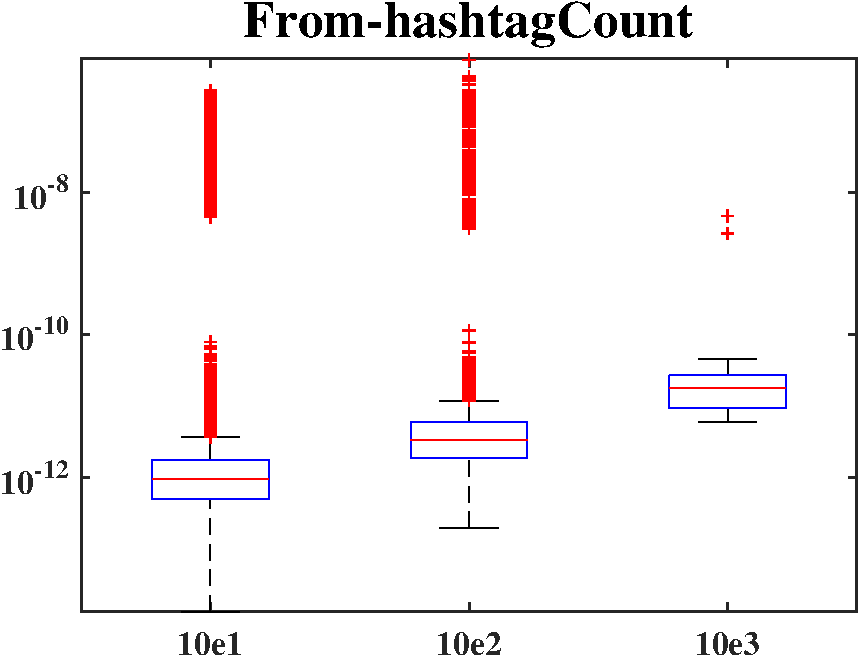
\includegraphics[width=32mm, height=35mm]{images/BoxPlots_IranDeal/From-hashtagCount.pdf}}
\subfloat[Fig:][Tweet Count]{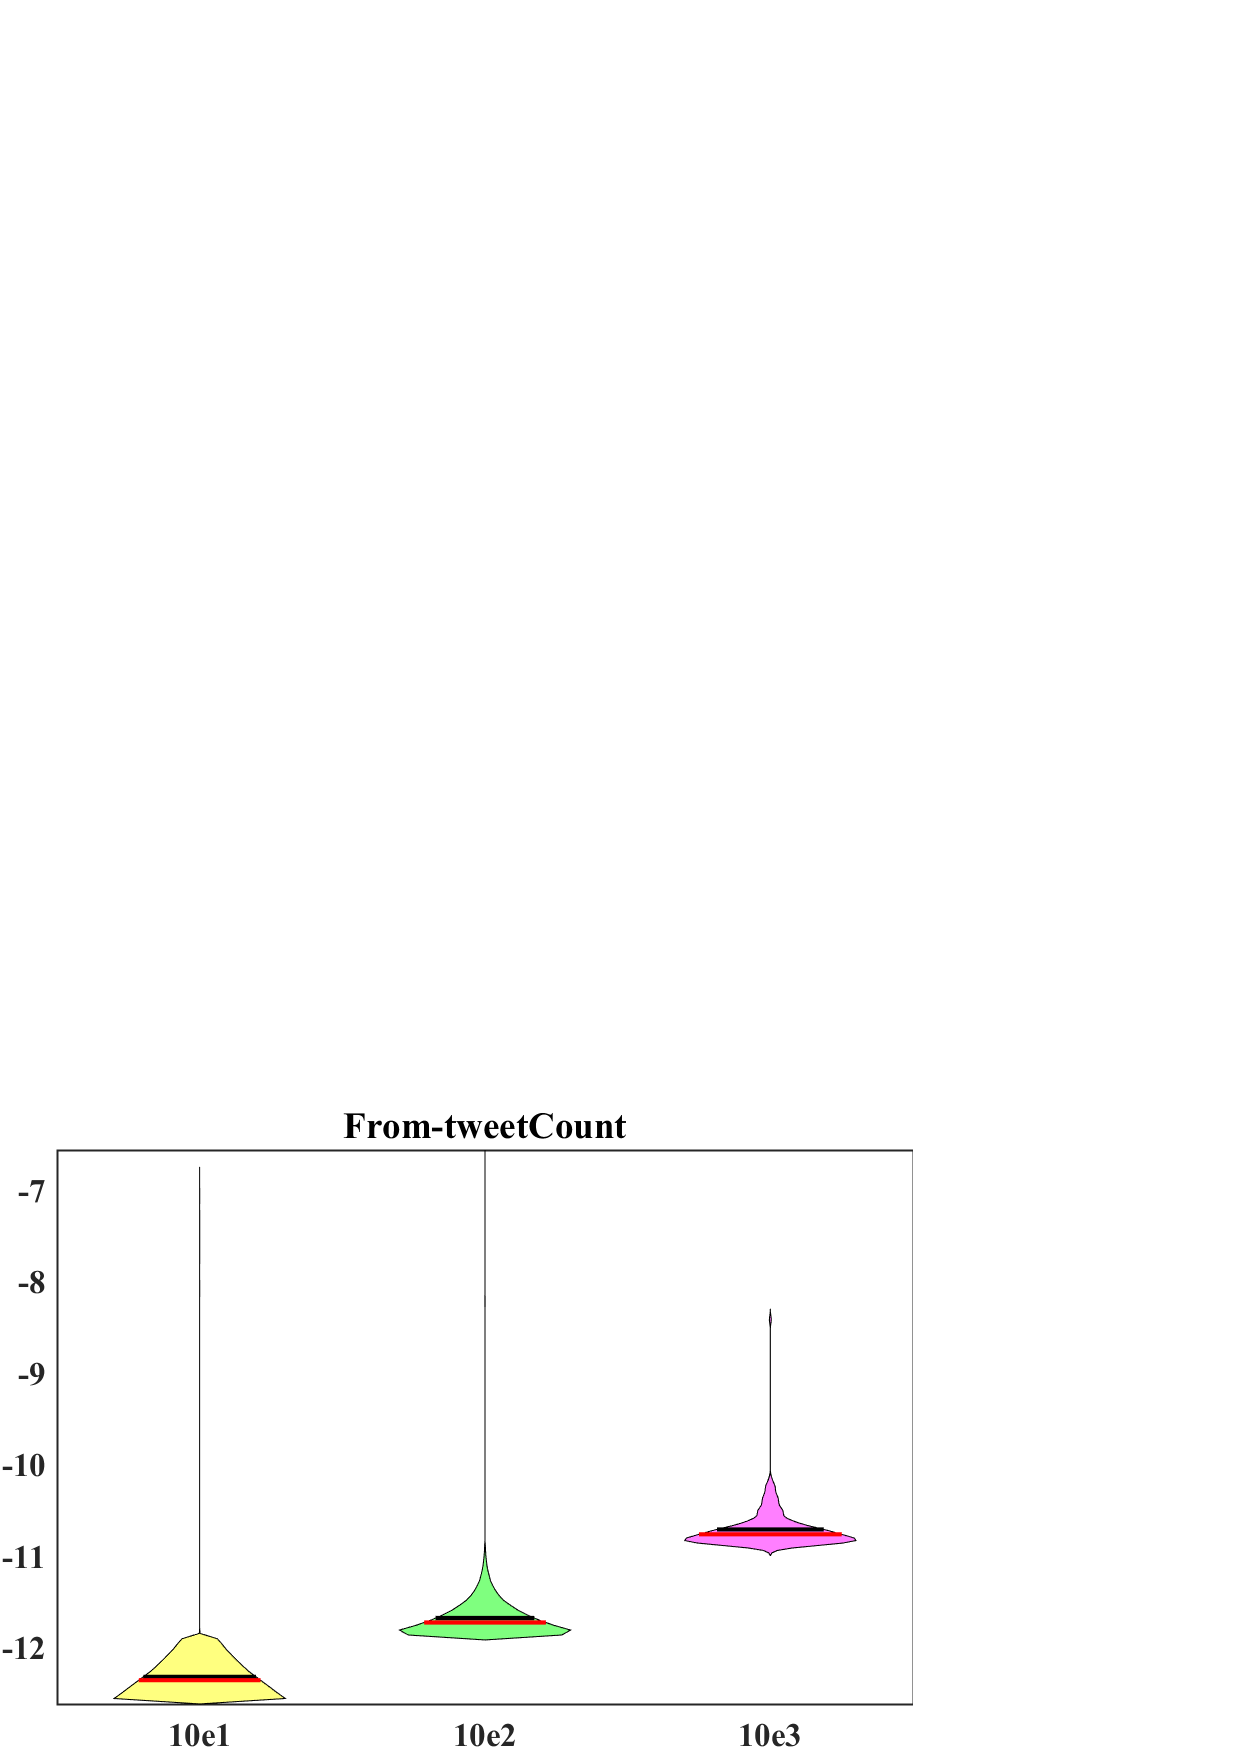
\includegraphics[width=32mm, height=35mm]{images/BoxPlots_IranDeal/From-tweetCount.pdf}} \\
%\vspace{-10mm}
\subfloat[Fig:][Tweet Count]{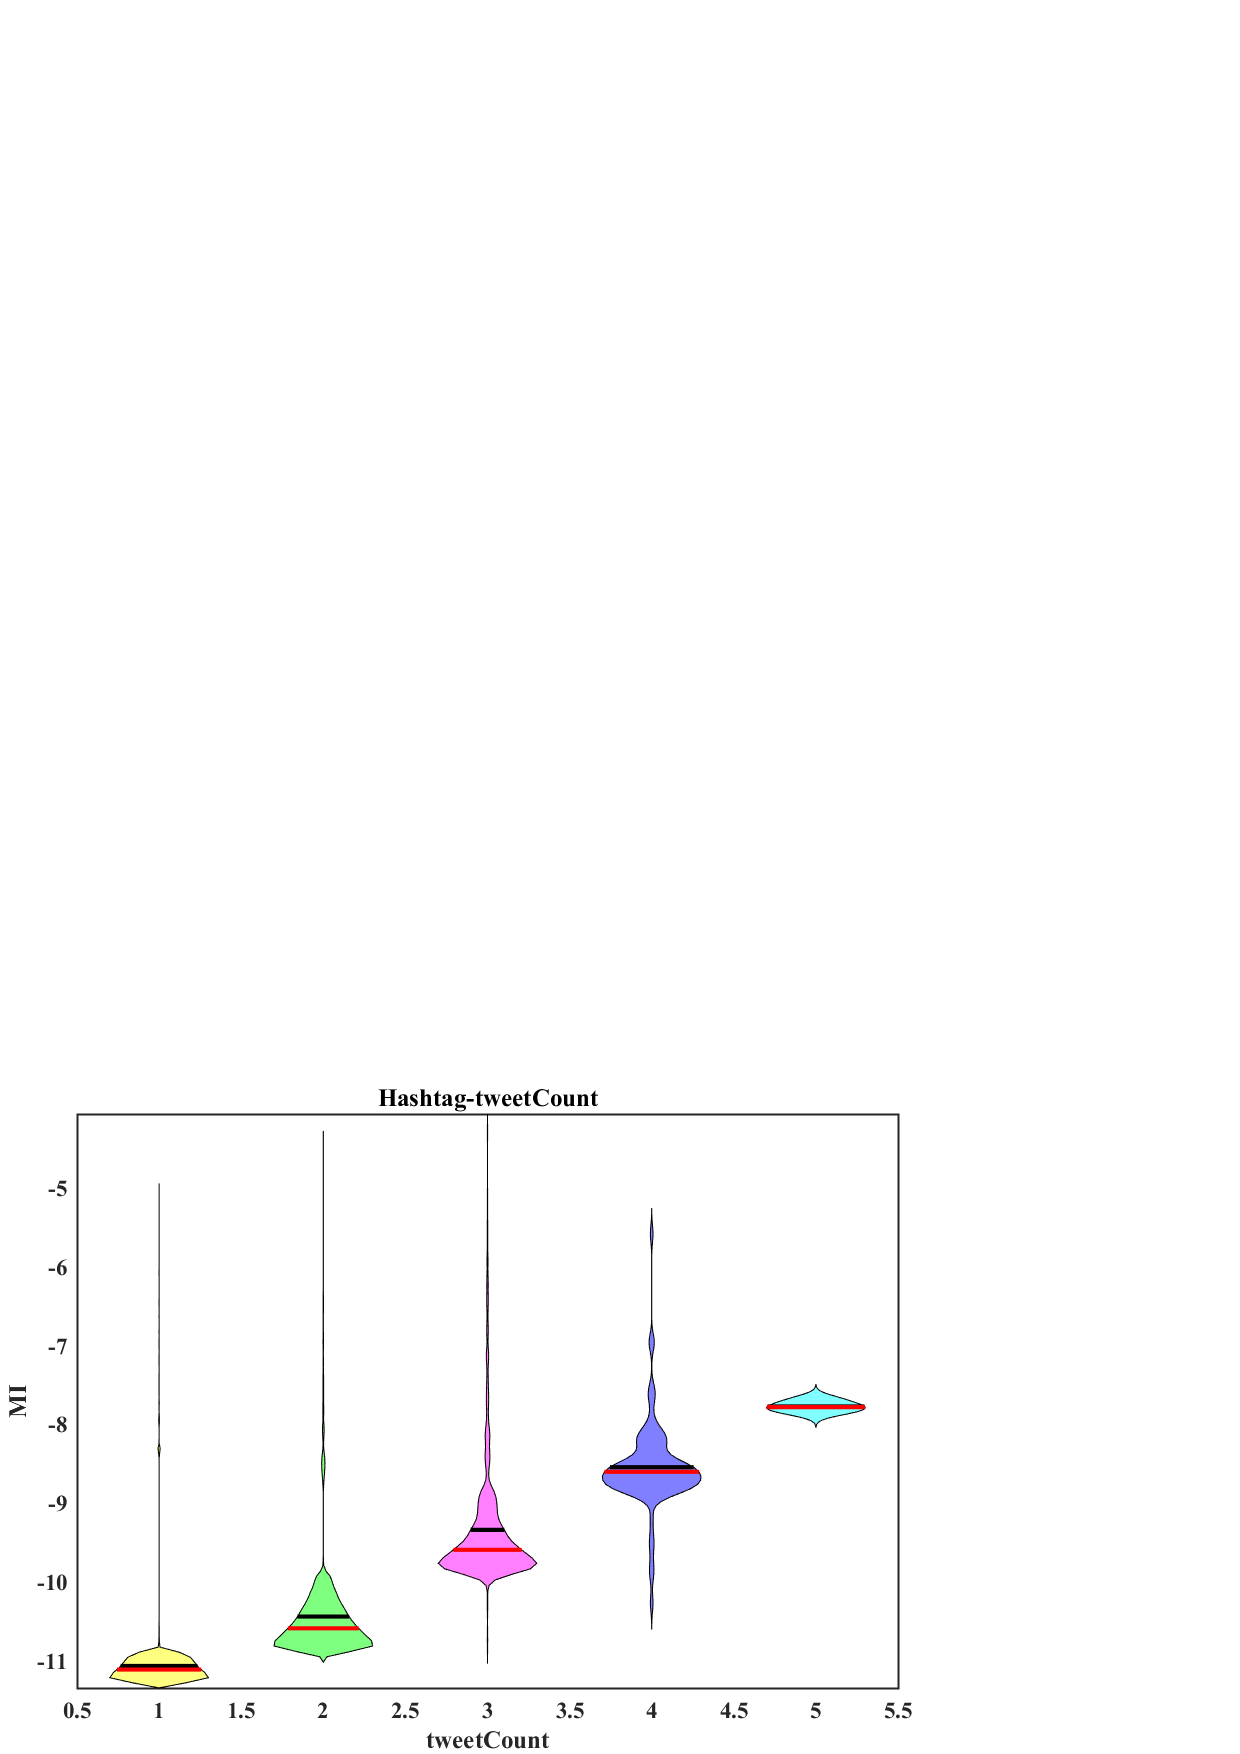
\includegraphics[width=32mm, height=35mm]{images/BoxPlots_IranDeal/Hashtag-tweetCount.pdf}}
\subfloat[Fig:][User Count]{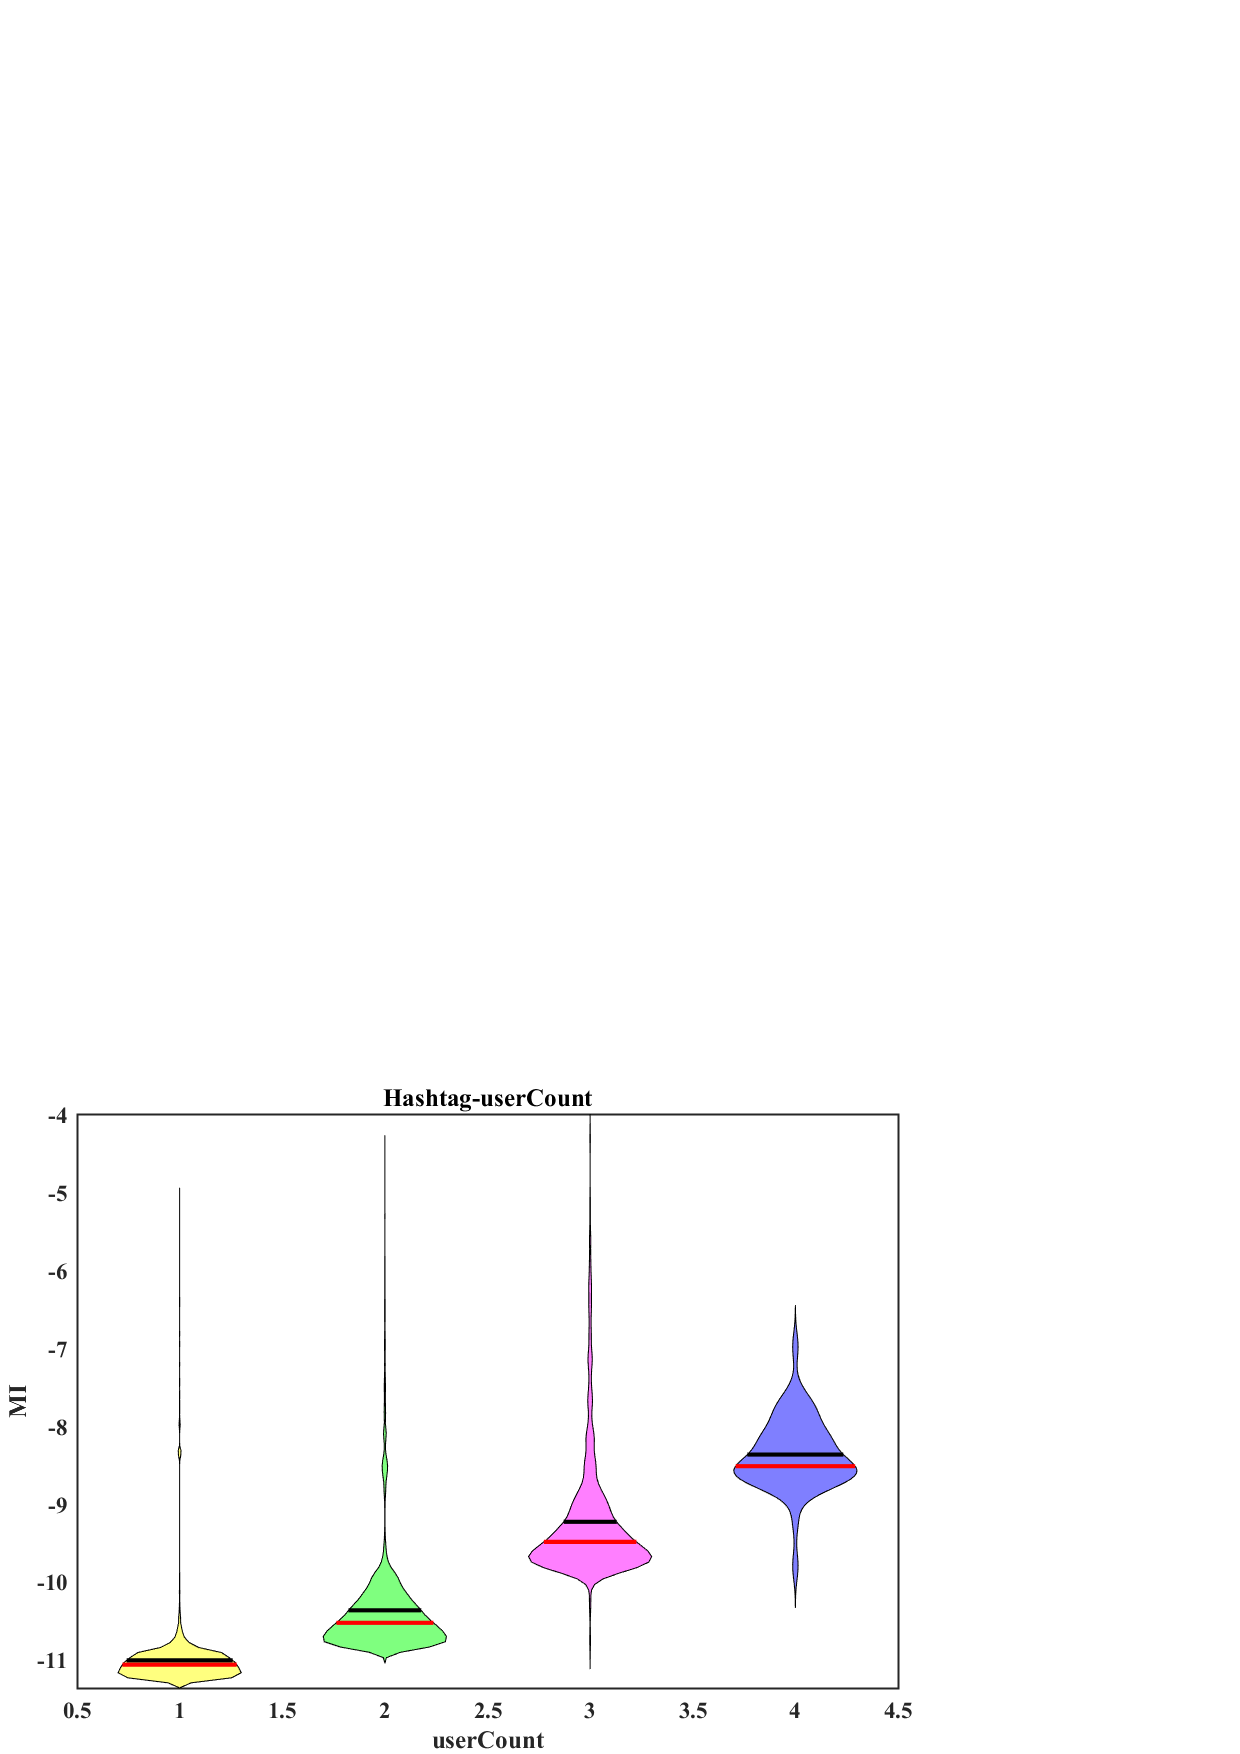
\includegraphics[width=32mm, height=35mm]{images/BoxPlots_IranDeal/Hashtag-userCount.pdf}}
\subfloat[Fig:][User Count]{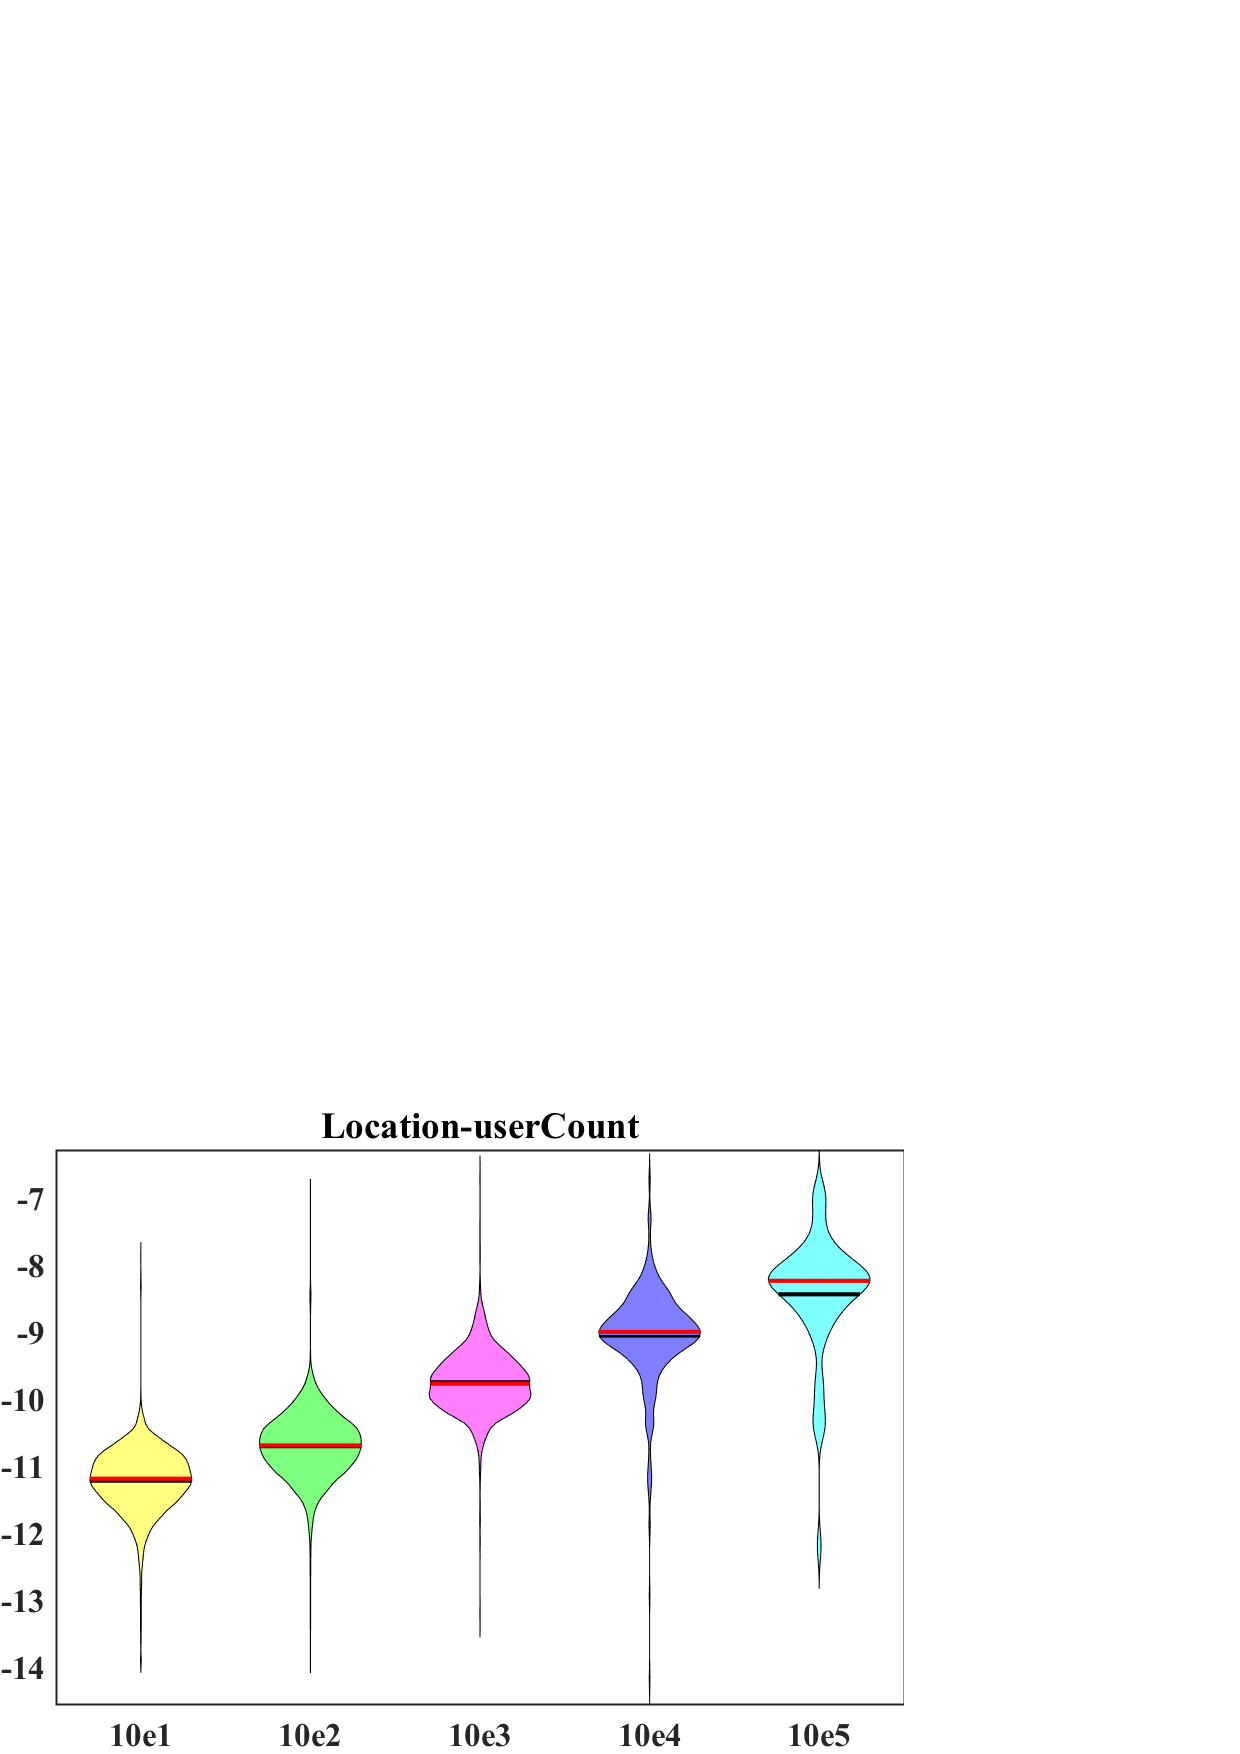
\includegraphics[width=32mm, height=35mm]{images/BoxPlots_IranDeal/Location-userCount.pdf}}
\subfloat[Fig:][Tweet Count]{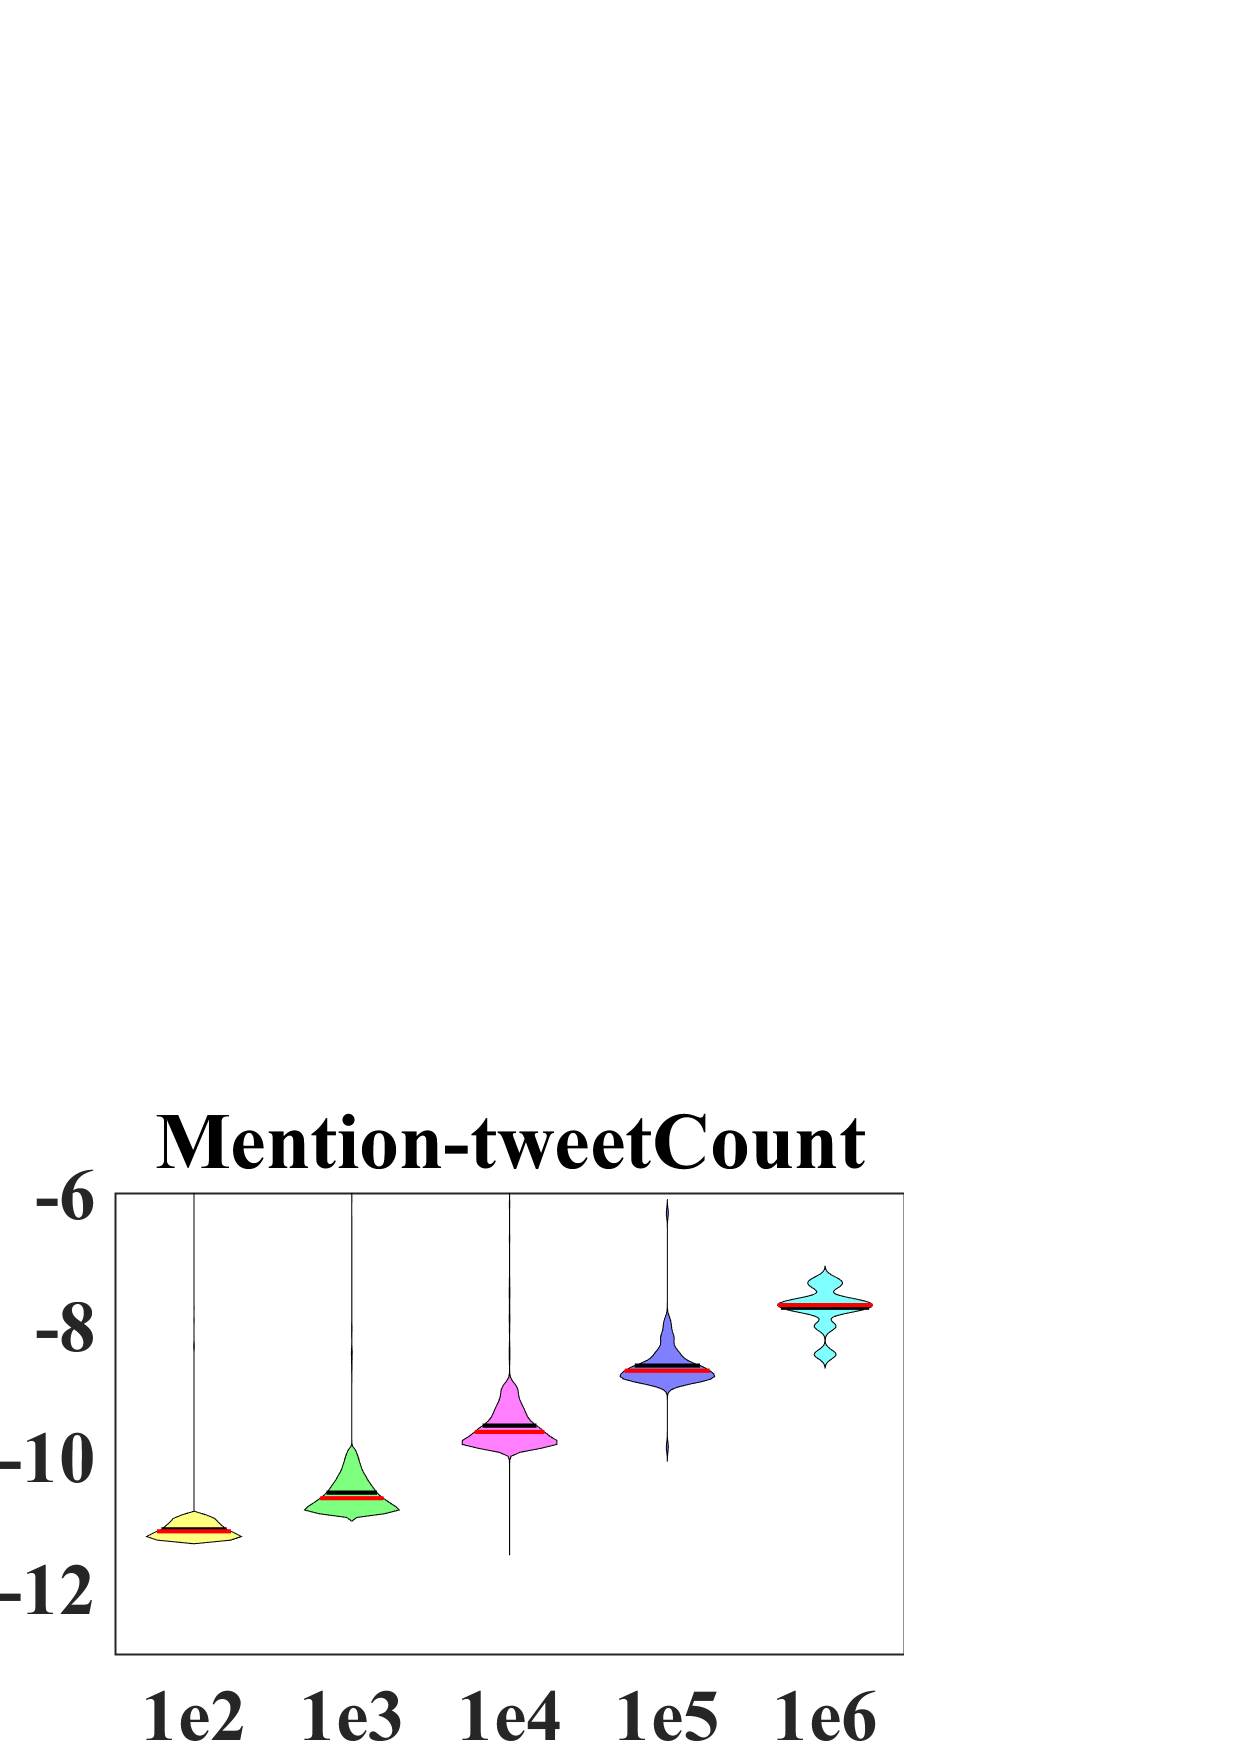
\includegraphics[width=32mm, height=35mm]{images/BoxPlots_IranDeal/Mention-tweetCount.pdf}}
\subfloat[Fig:][Tweet Count]{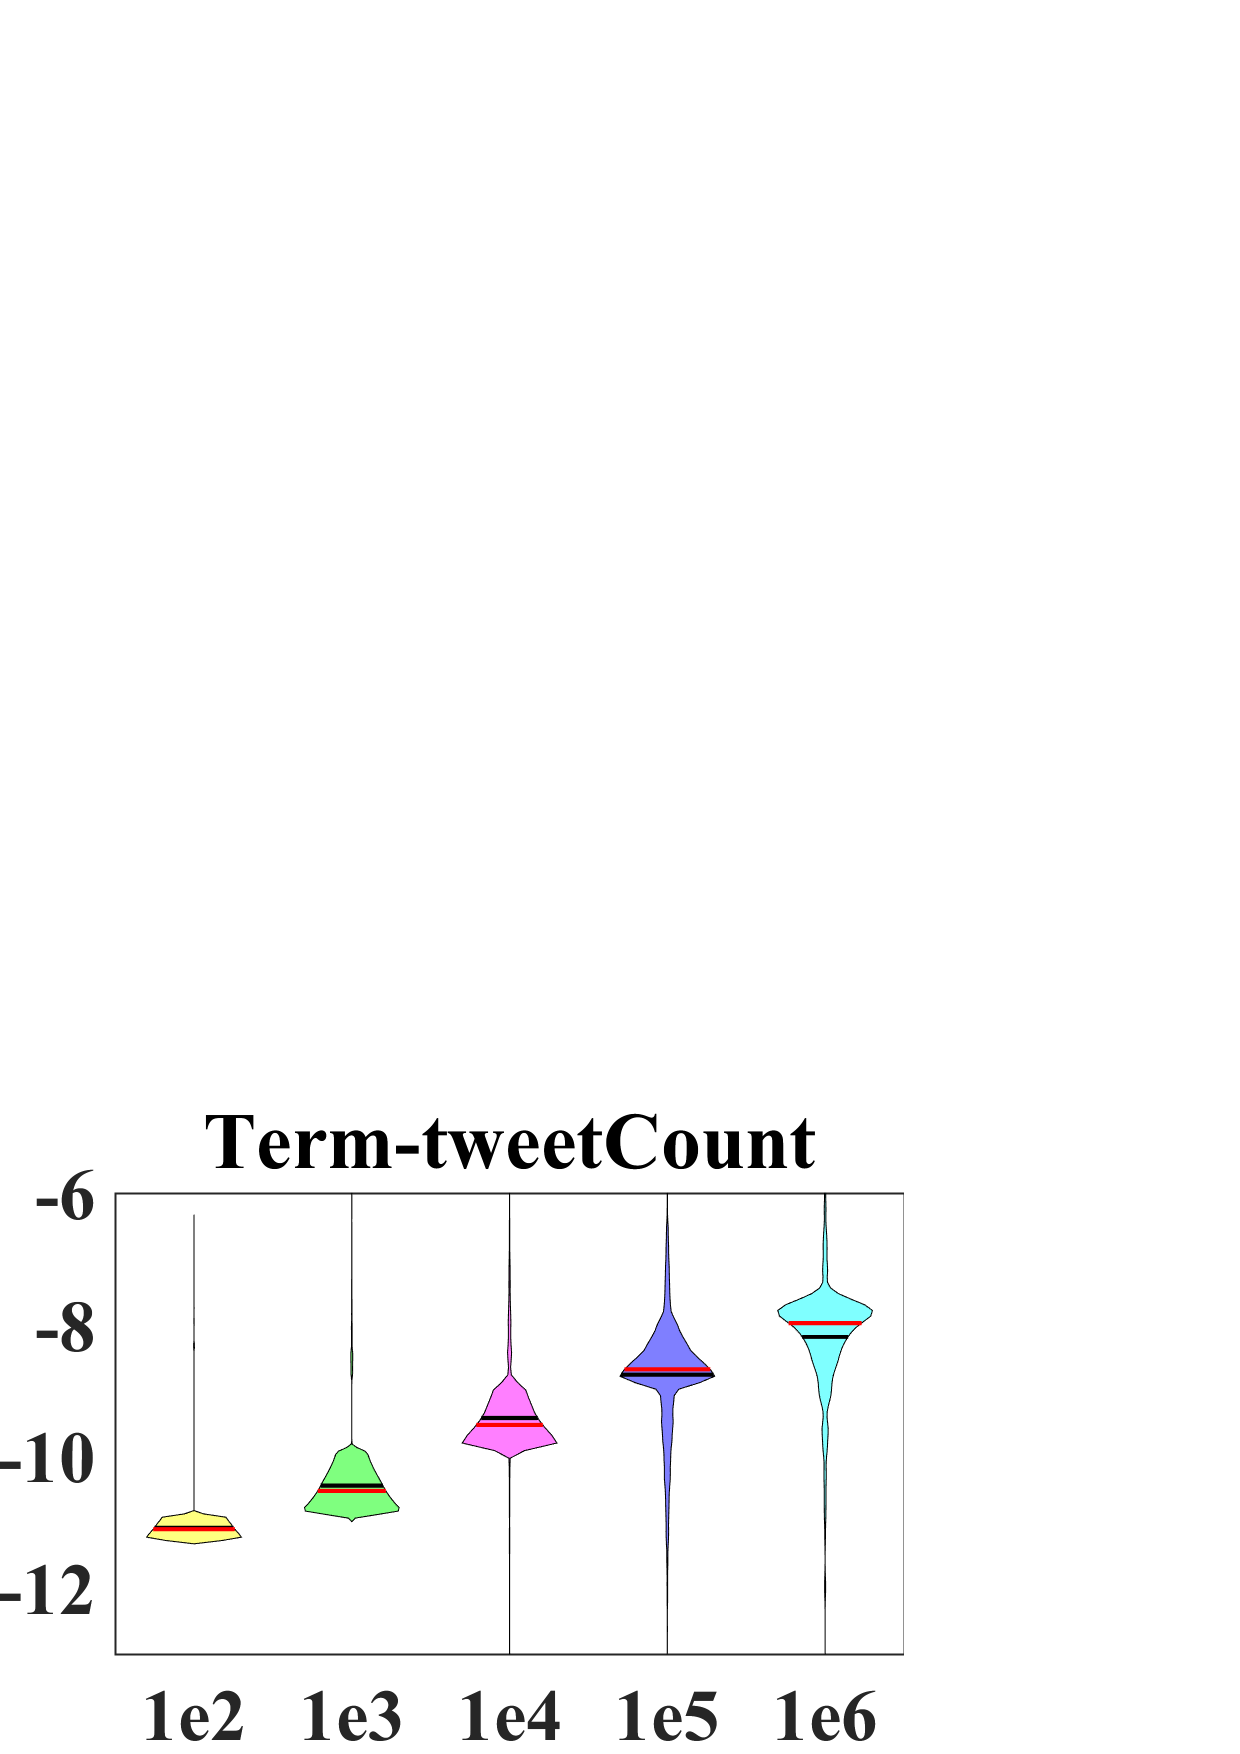
\includegraphics[width=32mm, height=35mm]{images/BoxPlots_IranDeal/Term-tweetCount.pdf}} \\
\end{tabular}
\end{tabular}
\vspace{-2mm}
\caption {Box Plots for feature attributes counts vs. MI. Top row shows attributes \{favoriteCount, followerCount, friendCount, hashtagCount, tweetCount\} for $From$ feature. Bottom row shows attributes tweetCount and/or userCount for $Hashtag$, $Location$, $Mention$,and $Term$ features.}
\label{fig:boxplots2}
\end{figure*}
\fi
%%%%%%%%%%%%%%%%%%%%%%%%%%%%%%%%%%%%%%%%%%%%%%%%%%%%%%%%%%%%%%%%%%%%%%%%%%%


%%%%%%%%%%%%%%%%%%%%%%%%%%%%%%%%%%%%%%%%%%%%%%%%%%%%%%%%%%%%%%%%%%%%%%%%%%%
\begin{figure*}[tbph!]
\centering
\begin{tabular}{ccccc}
\begin{tabular}{ccccc}
\subfloat[Fig:][]{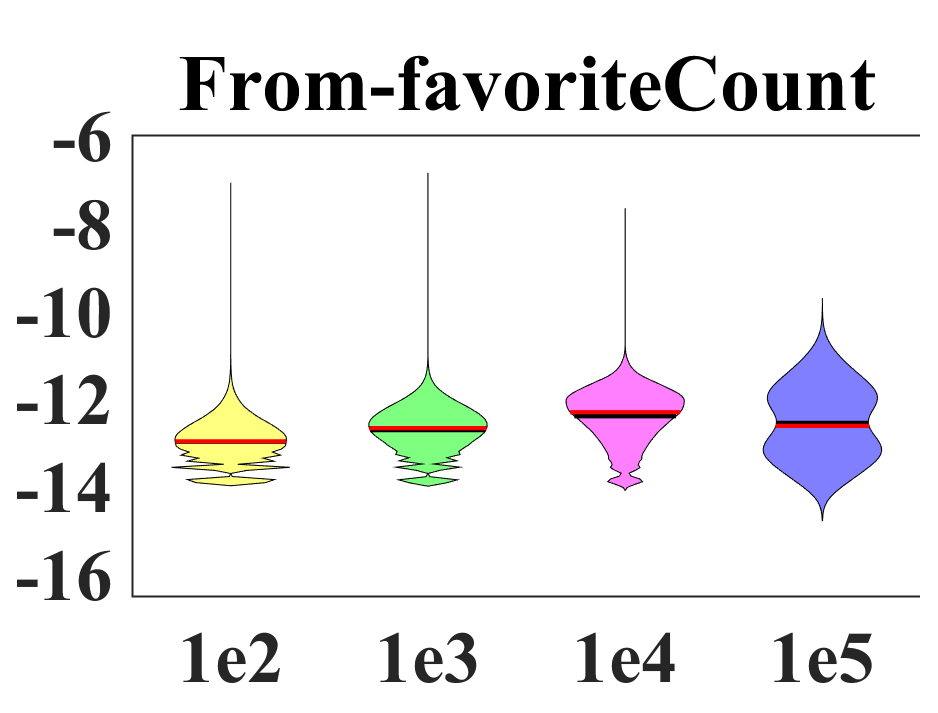
\includegraphics[width=32mm, height=35mm]{images/ViolinPlots/From-favoriteCount.eps}}
\subfloat[Fig:][]{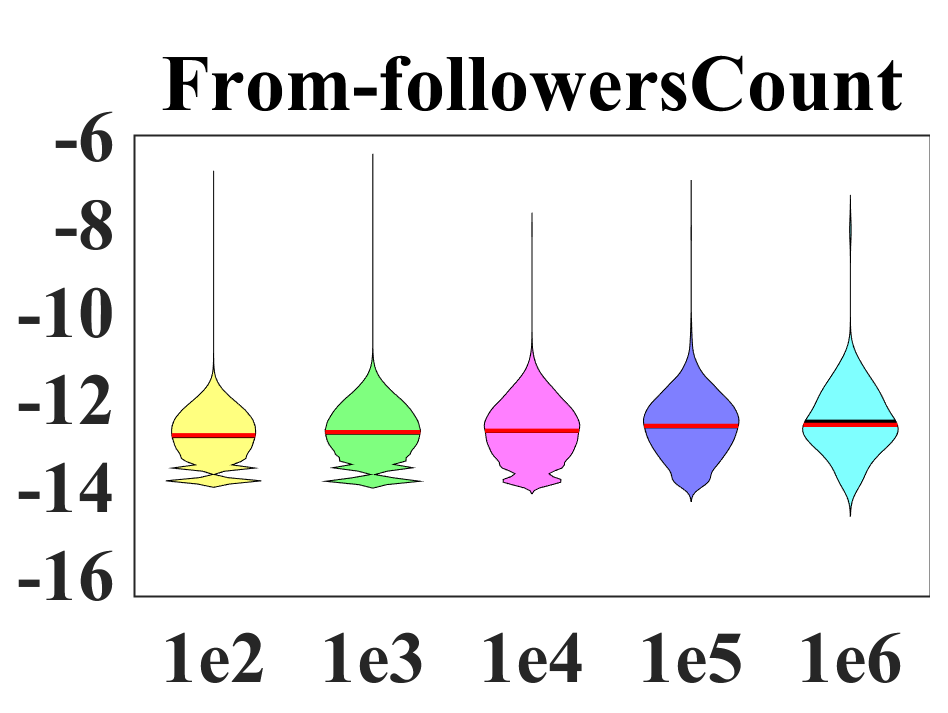
\includegraphics[width=32mm, height=35mm]{images/ViolinPlots/From-followersCount.eps}}
\subfloat[Fig:][]{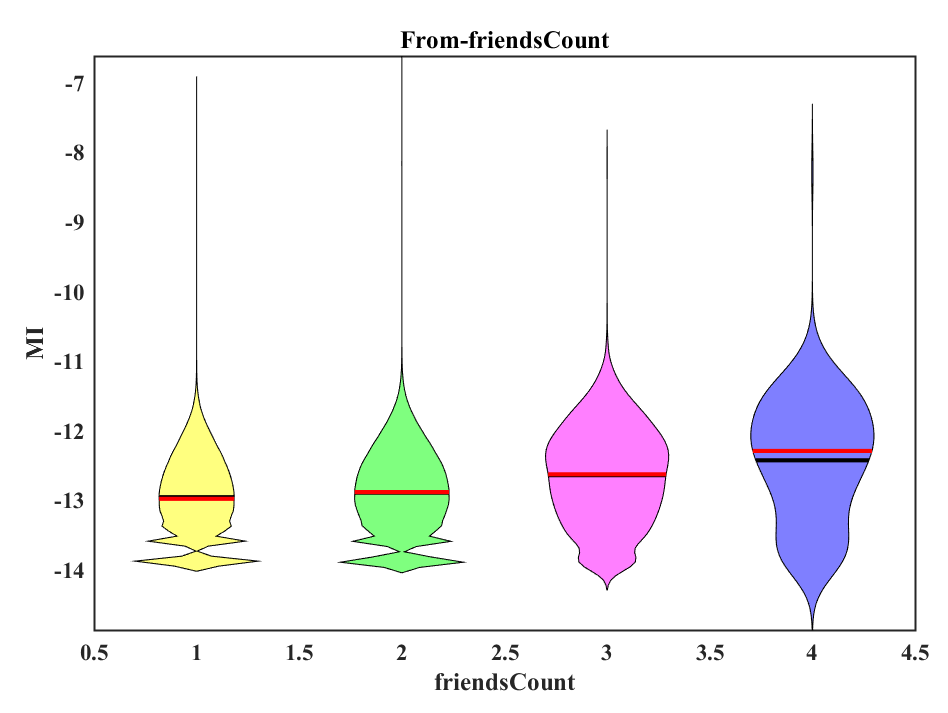
\includegraphics[width=32mm, height=35mm]{images/ViolinPlots/From-friendsCount.eps}}
\subfloat[Fig:][]{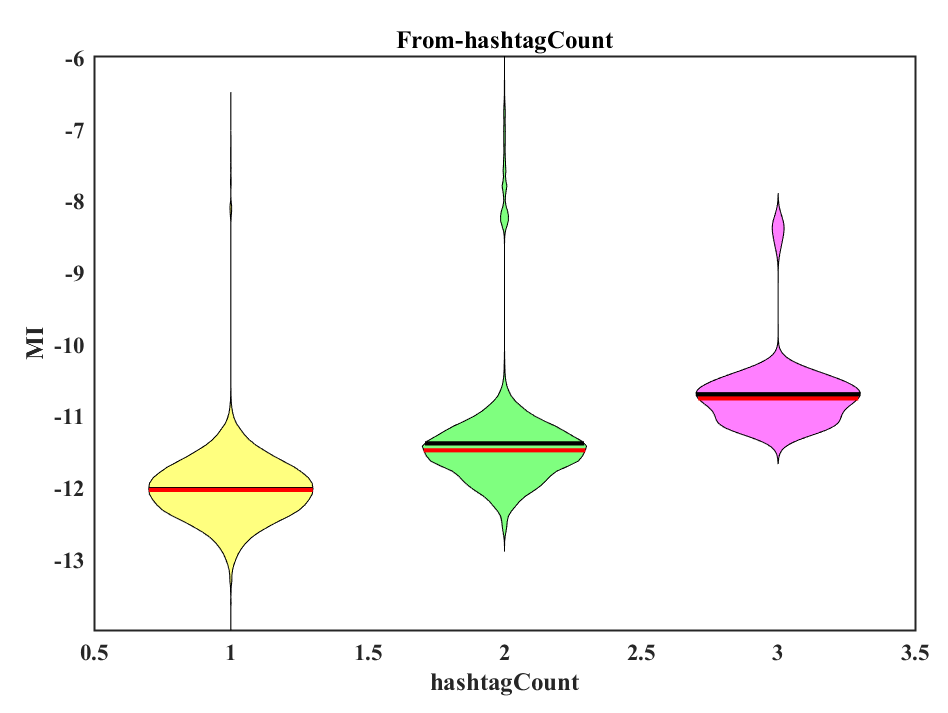
\includegraphics[width=32mm, height=35mm]{images/ViolinPlots/From-hashtagCount.eps}}
\subfloat[Fig:][]{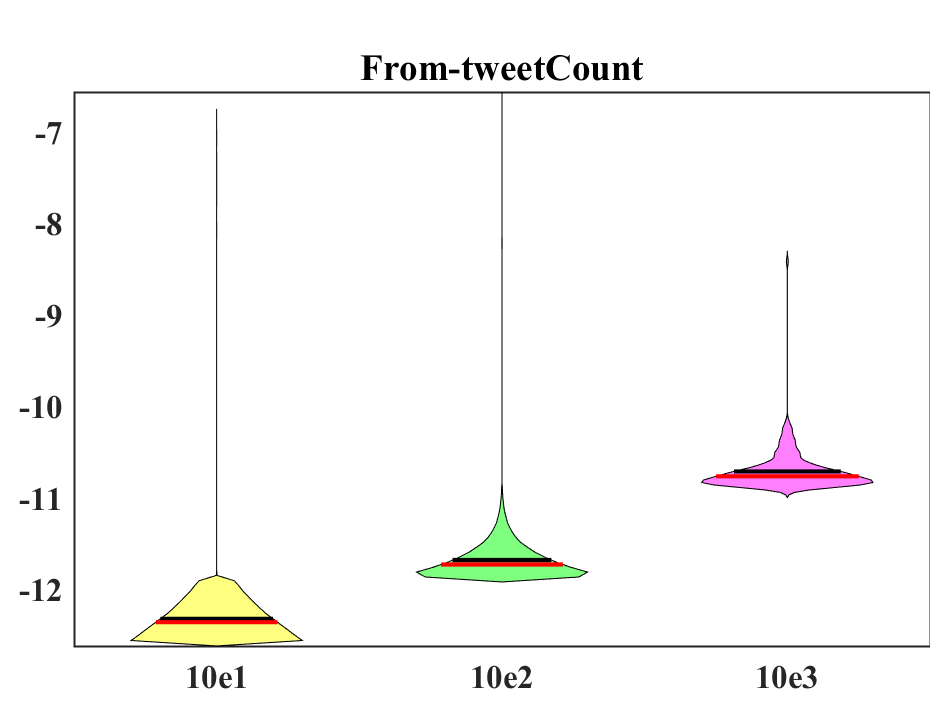
\includegraphics[width=32mm, height=35mm]{images/ViolinPlots/From-tweetCount.eps}} \\
%\vspace{-10mm}
\subfloat[Fig:][]{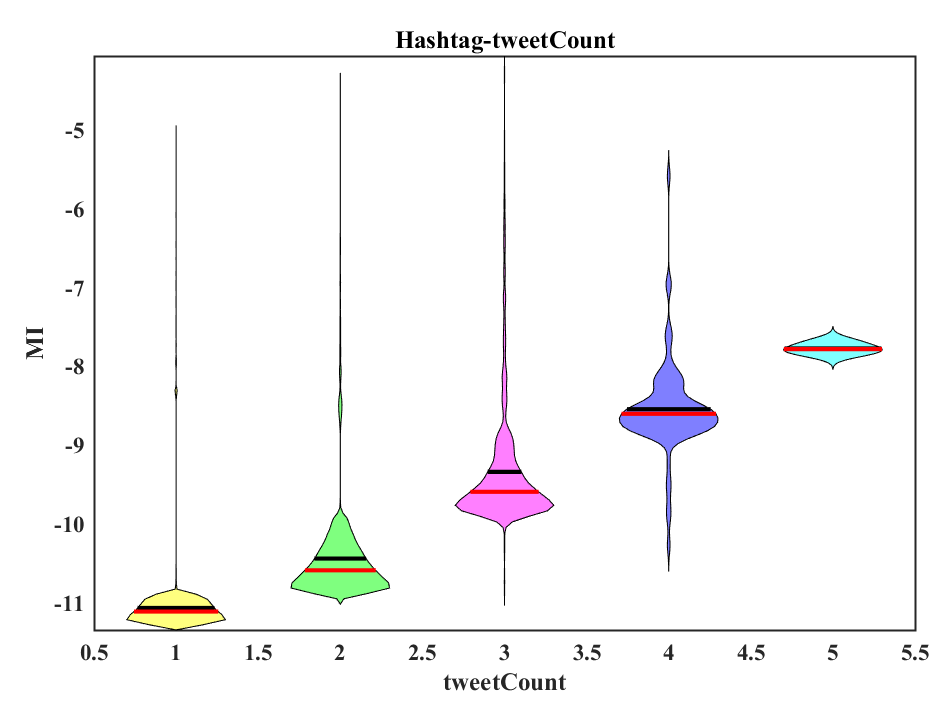
\includegraphics[width=32mm, height=35mm]{images/ViolinPlots/Hashtag-tweetCount.eps}}
\subfloat[Fig:][]{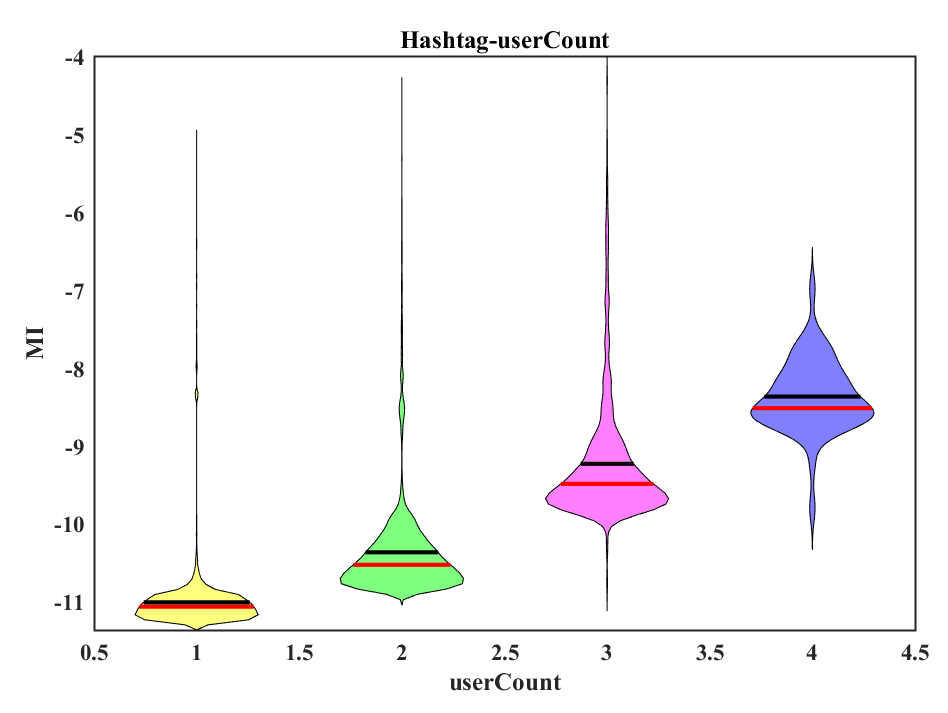
\includegraphics[width=32mm, height=35mm]{images/ViolinPlots/Hashtag-userCount.eps}}
\subfloat[Fig:][]{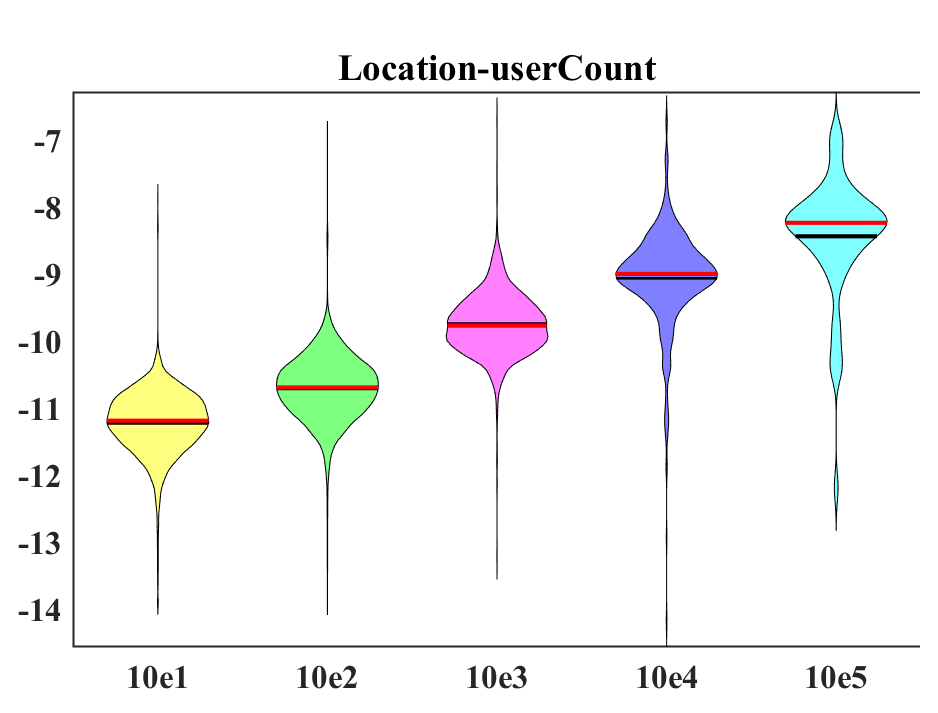
\includegraphics[width=32mm, height=35mm]{images/ViolinPlots/Location-userCount.eps}}
\subfloat[Fig:][]{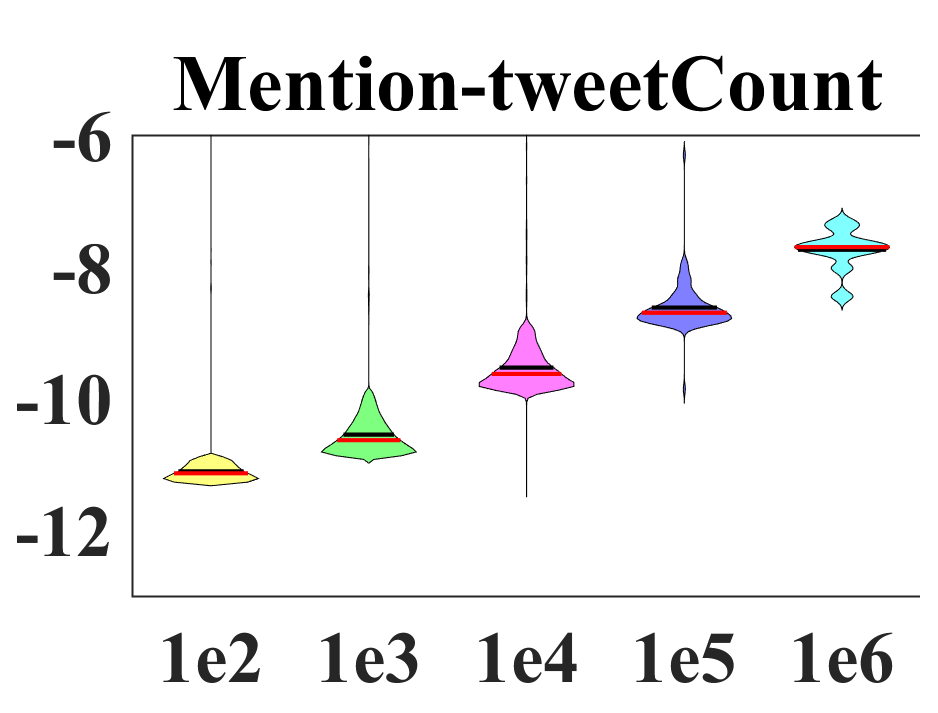
\includegraphics[width=32mm, height=35mm]{images/ViolinPlots/Mention-tweetCount.eps}}
\subfloat[Fig:][]{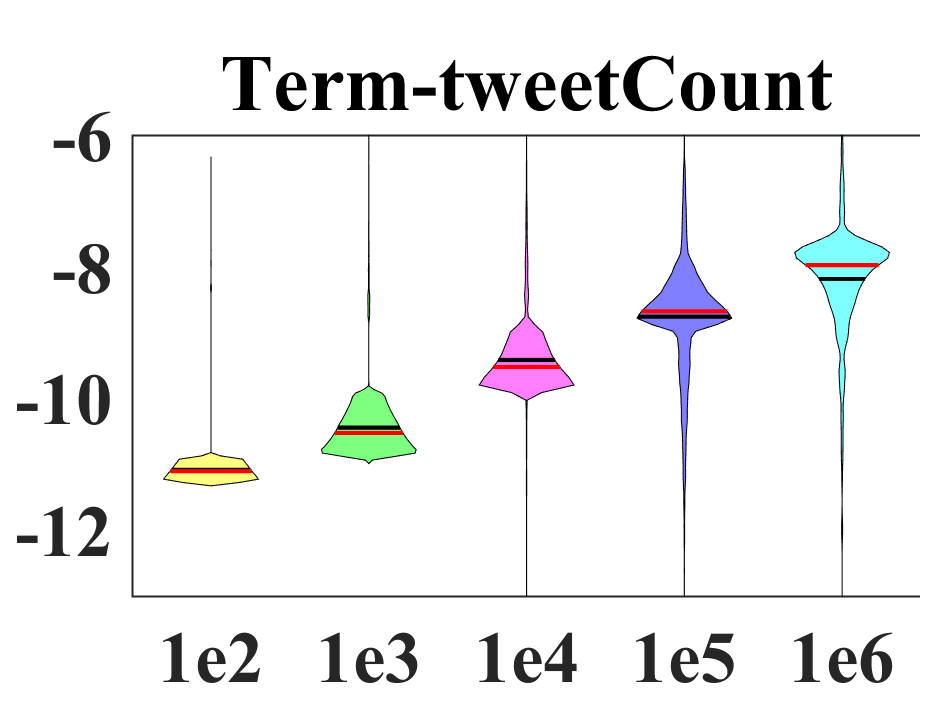
\includegraphics[width=32mm, height=35mm]{images/ViolinPlots/Term-tweetCount.eps}} \\
\end{tabular}
\end{tabular}
\vspace{-2mm}
\caption {ViolinPlots for feature attributes counts vs. MI. Top row shows attributes \{favoriteCount, followerCount, friendCount, hashtagCount, tweetCount\} for $From$ feature. Bottom row shows attributes tweetCount and/or userCount for $Hashtag$, $Location$, $Mention$,and $Term$ features.}
\label{fig:violinplots}
\end{figure*}
%%%%%%%%%%%%%%%%%%%%%%%%%%%%%%%%%%%%%%%%%%%%%%%%%%%%%%%%%%%%%%%%%%%%%%%%%%%


%%%%%%%%%%%%%%%%%%%%%%%%%%%%%%%%%%%%%%%%%%%%%%%%%%%%%%%%%%%%%%%%%%%%%%%%%%%
\begin{figure*}[tbph!]
\centering
\begin{tabular}{cccc}
\subfloat[Fig:][]{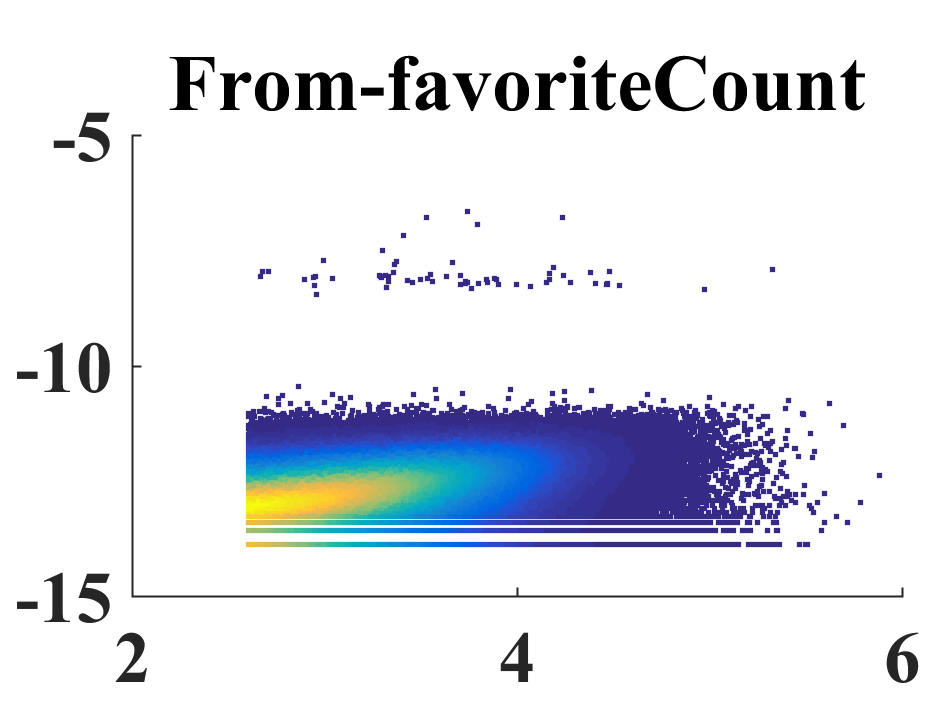
\includegraphics[width=40mm, height=35mm]{images/DensityPlots_IranDeal/dscatterPlot_From-favoriteCount.eps}} \qquad
\subfloat[Fig:][]{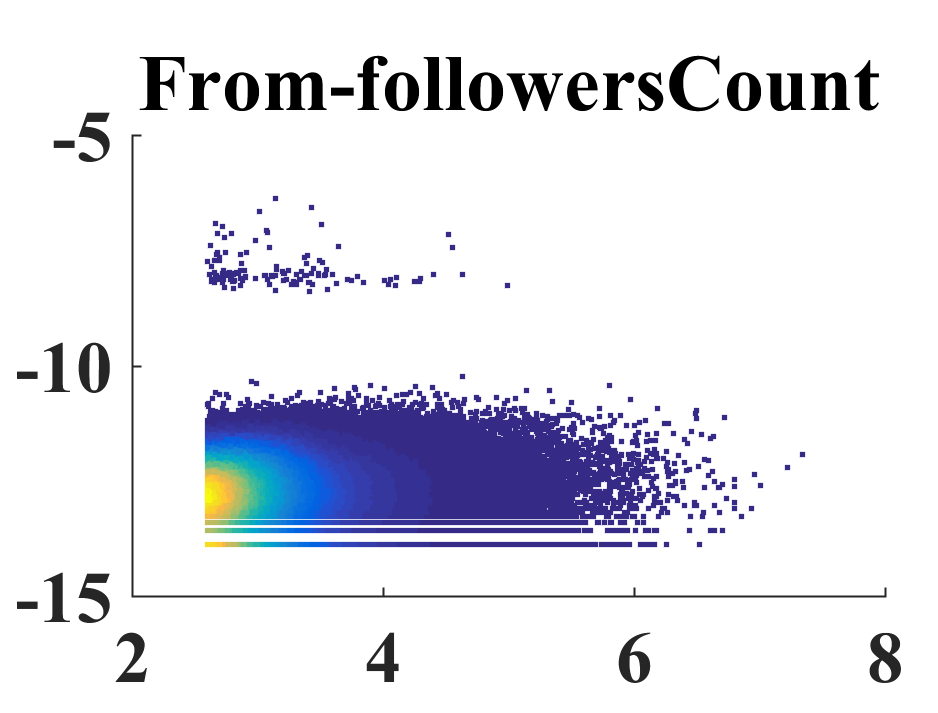
\includegraphics[width=40mm, height=35mm]{images/DensityPlots_IranDeal/dscatterPlot_From-followersCount.eps}} \qquad
\subfloat[Fig:][]{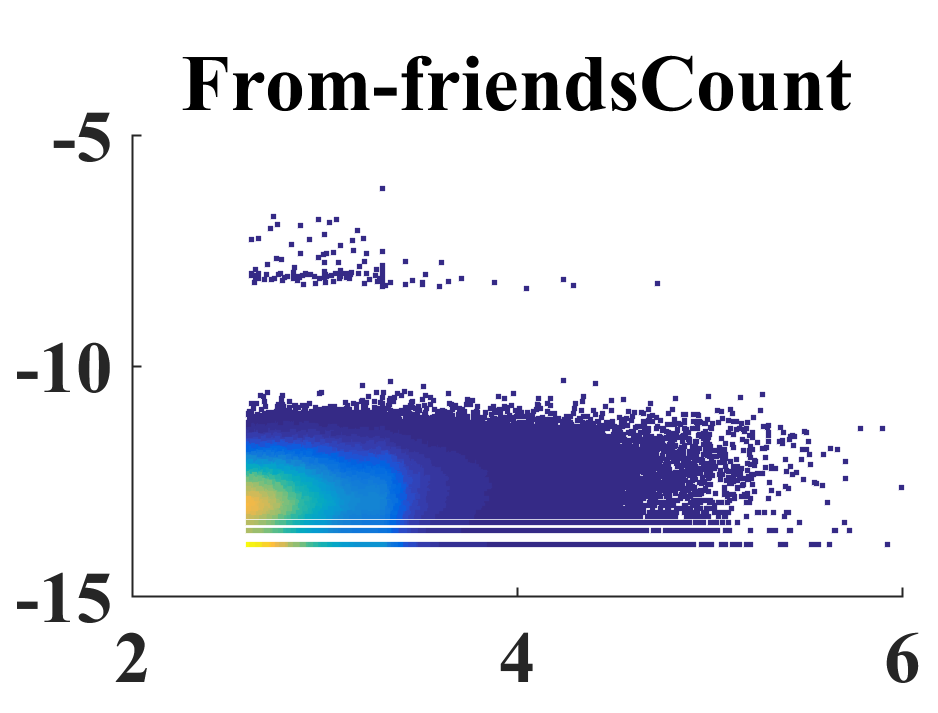
\includegraphics[width=40mm, height=35mm]{images/DensityPlots_IranDeal/dscatterPlot_From-friendsCount.eps}} \qquad
\subfloat[Fig:][]{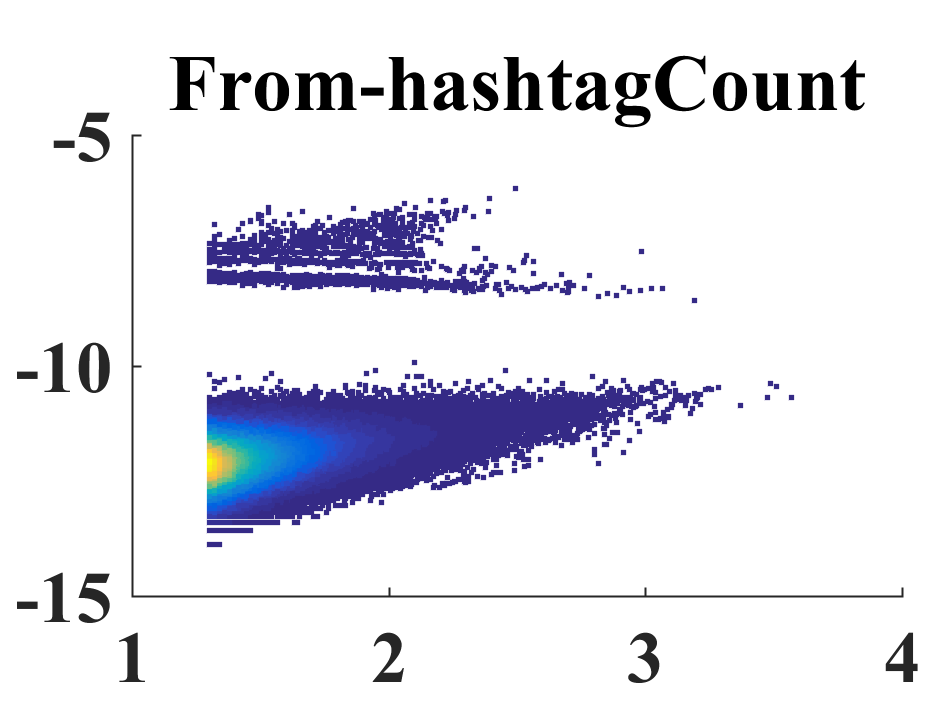
\includegraphics[width=40mm, height=35mm]{images/DensityPlots_IranDeal/dscatterPlot_From-hashtagCount.eps}} \\
\end{tabular}
\vspace{-2mm}
\caption {DensityPlots for feature attributes counts vs. MI. (a-d) show attributes \{favoriteCount, followerCount, friendCount, hashtagCount\} for $From$ feature}
\label{Fig3}
\end{figure*}
%%%%%%%%%%%%%%%%%%%%%%%%%%%%%%%%%%%%%%%%%%%%%%%%%%%%%%%%%%%%%%%%%%

\section{Conclusions and Future Work}
This work fills a major gap in 
event detection and tracking from social media
on identifying emerging topics from long-running themes with
minimal user supervision.  Our results suggest that these
sensors generalize well to unseen future topical content and provide a
novel paradigm for the extraction of high-value content from social
media.  Future work should explore the following enhanced topical
social sensor learning tasks: (1) optimizing rankings not only for topicality
but also to minimize the lag-time of novel content identification, (2) optimizing
queries for boolean retrieval oriented APIs such as Twitter, and (3) utilizing 
more social network structure to exploit a more expressive graph-based features.


% No identifying information in submitted version. -SPS
%\section{Acknowledgments}
%We thank Dan Nguyen for his help with data processing.
%We thank Kanna for her assistance in curating the topical hashtags in the Twitter data used in this study.
%
%\section{Copyright}

\bibliographystyle{aaai}
\bibliography{bibliography.bib}

\end{document}
